%\chapter{Kinematic Corrections}
\section{Kinematic Corrections}
\label{cha:KineCor}
The reconstructed event vertices and associated particle 4-momenta are slightly off from their true values for several reasons. First, % of all, %SEK
RECSIS does not take into account the fact that the beam is rastered in polarized target experiments. Next, any 
imperfections and mis-alignments of detectors and other components of the experimental set-up are not accounted for. 
Furthermore, the torus field map is not known precisely. 
In addition, the effects of multiple-scattering and particle energy losses are not considered in RECSIS. %Finally, RECSIS itself has imperfections inherent in its algorithm. %SEK: Unless you want to explain, leave out.
Therefore, to get more accurate results from the data analysis, the data quality must be improved by applying various kinematic corrections. Following is the list of the corrections that were applied for %is applied for each particle from our data 
the analysis:

\begin{enumerate}
\item Incoming (beam) energy loss correction (due to ionization) 
\item Tracking corrections
%%%%\begin{enumerate}
%%%%\item Beam off-set correction % equivalent to Raster correction?
%\item Drift chamber dependent momentum correction
%\item Z-vertex correction
%%%%\item Solenoid axis tilt correction
%%%%\item Solenoid axis offset correction
%%%%\end{enumerate}
%\item Stray magnetic field correction 
\item Drift chamber dependent momentum correction
%\item Multiple scattering correction (Not considered because, we are looking at electron-only inclusive events)
\item Outgoing energy loss correction (due to ionization after scattering) %/reaction))
\end{enumerate}



%\section{Incoming Energy Loss Correction}
\subsection{Incoming Energy Loss Correction}
%Out of these corrections, the first one
The first correction listed above considers the loss of beam energy due to atomic collisions before the actual nuclear scattering takes place. %As an adjustment for the loss, an estimate of 2 MeV
A good estimate for this loss is 2 MeV on average \cite{pComKuhn, pComBosted}, which is subtracted from the nominal beam energy. This correction is applied during the analysis whenever the beam energy is involved\footnote{The beam energies that we used were derived from the Hall A and Hall C Tiefenback energies  or the MDSY1c or MDSY3c energies\cite{eg4Ebeam}}, %For more info, read X. Zheng's analysis note around page 35.
and therefore it is not included in the correction package described below.





%\section{Raster Correction}

%This section still being expanded ... \newline \newline

%\subsubsection{Beam Rastering in Hall-B Polarized target Experiments}


The polarized electron beam coming from CEBAF to Hall B is rastered in polarized target experiments. This 
is done to minimize radiation damage (depolarizing effects) to the polarized target and also to make maximum use of 
the target material (effective beam size increases and, therefore, the overall volume of exposed target increases). 
The beam is periodically spiraled covering a circular region of the target cross-section by using two raster 
magnets - one for the horizontal (X) direction and the other for the vertical direction (Y). The currents driving 
the two magnets are continuously recorded by analog-to-digital converters (ADCs).

\begin{figure}[htpb] %ht, htpb (p - float, b = bottom, h=? t = top)
\centerline{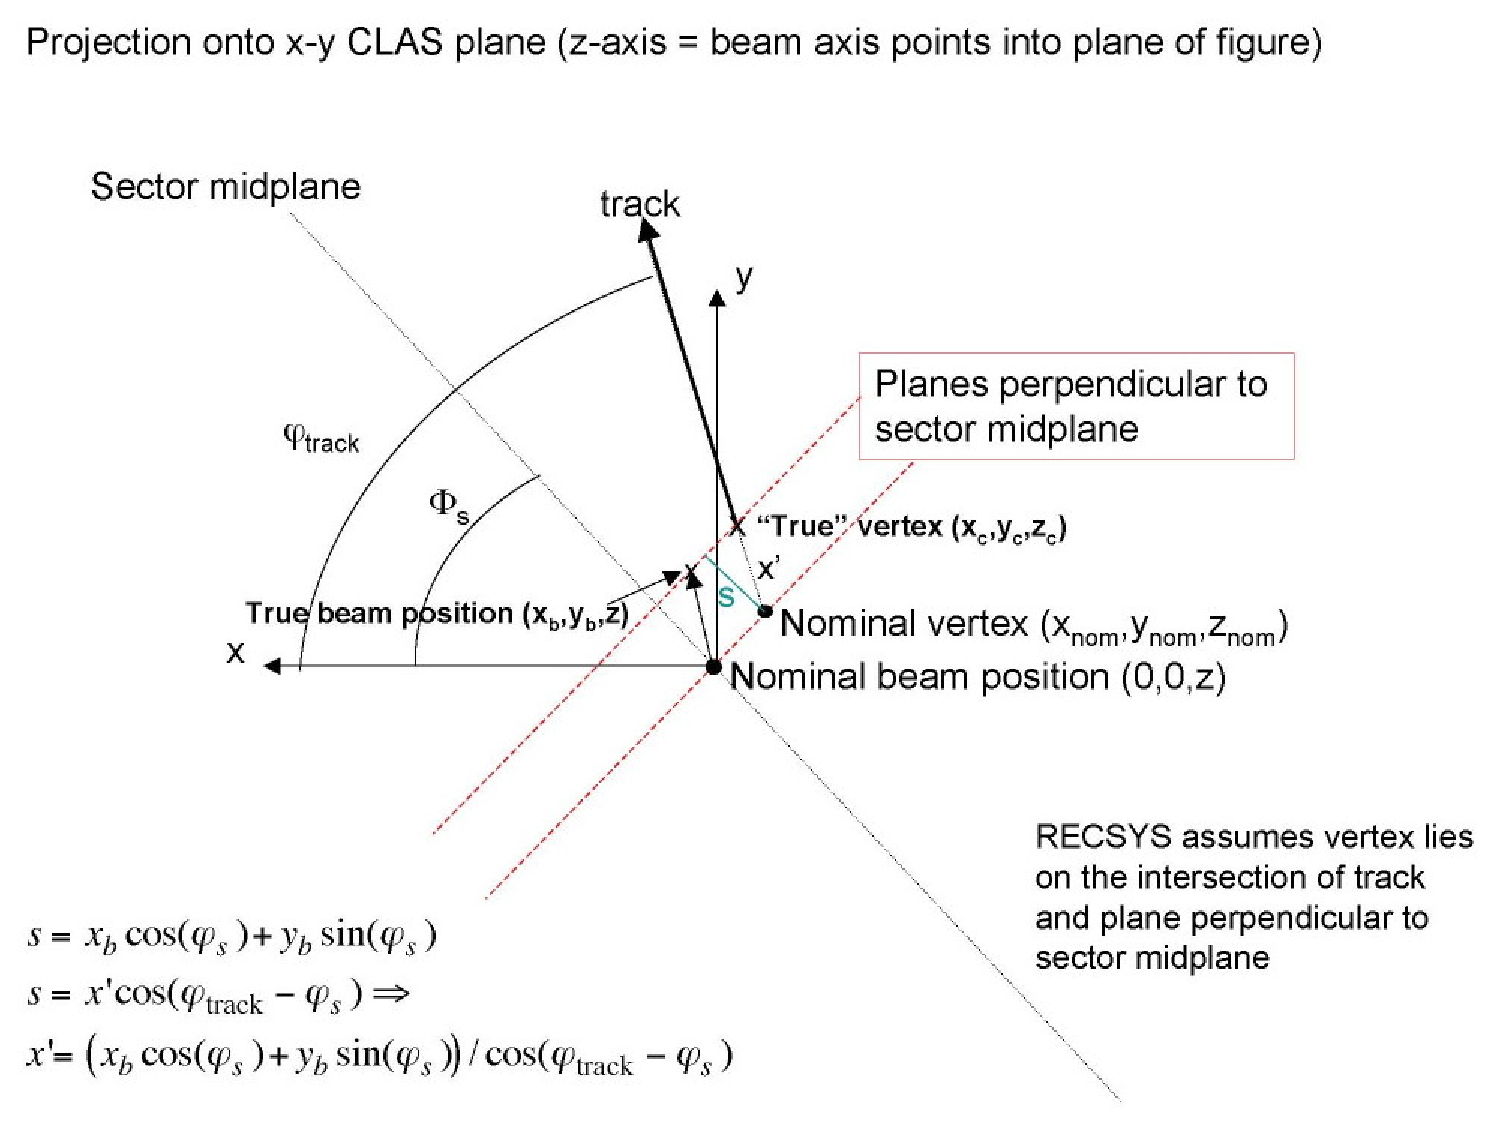
\epsfig{height=10cm,width=15cm,file=figuresEG4/FigKineCor/Raster_Corr_Formulae_Page_1.png}}
\caption{Raster correction geometry illustration (Figure courtesy of S. Kuhn)}
\label{fig:RstGeoKuhn1}
\end{figure}

The ADC values thus recorded can be translated to the coordinates (x,y) of the exact beam position at the target. The values of x,y can then be used to make corrections to the original track by RECSIS (which assumes x and y were zero), allowing better z-vertex and azimuthal angle ($\phi$) reconstruction. The better z-vertex reconstruction allows better selection of events from the target proper, rejecting events from upstream and downstream %up-beam and down-beam %GED
windows (especially for particles at small angles), and can also be used to reduce accidental coincidences in multi-particle final states (or to look for offset decays such as from $\Lambda$). Correction of $\phi$ improves missing mass resolution for multi-particle final states which is very important in exclusive channel analysis. In addition, plotting a two-dimensional histogram of events as a function of the raster information x and y, one can look for mis-steered beam that might have hit the target cup edges.

\begin{figure}[htpb] %ht, htpb (p - float, b = bottom, h=? t = top)
\centerline{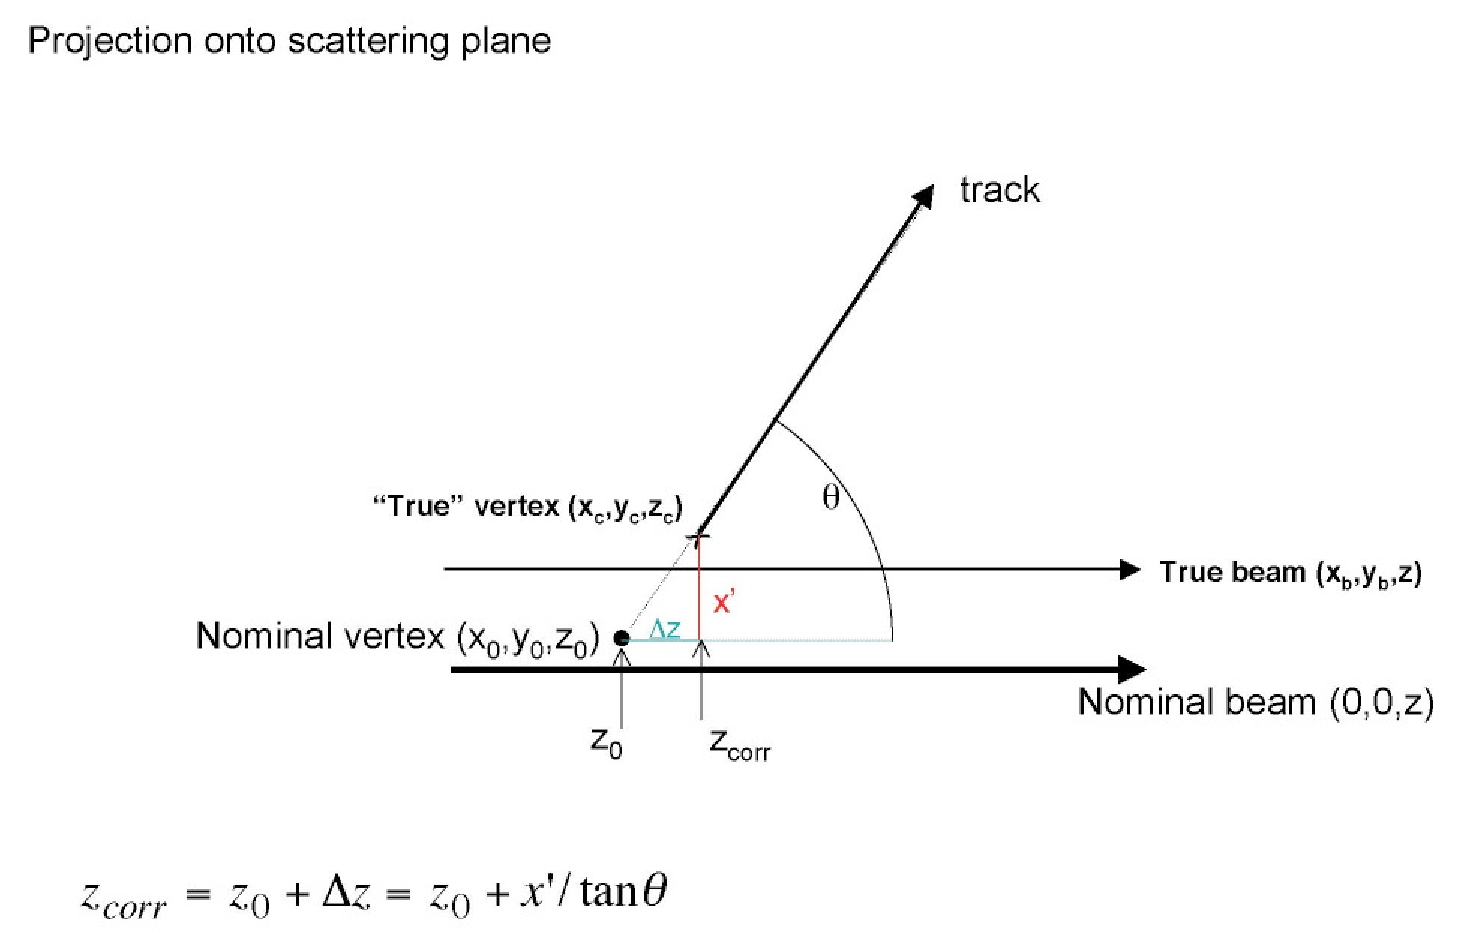
\epsfig{height=10cm,width=15cm,file=figuresEG4/FigKineCor/Raster_Corr_Formulae_Page_2.png}}
\caption{Raster correction geometry illustration (Figure courtesy - S. Kuhn)}
\label{fig:RstGeoKuhn2}
\end{figure}

A procedure was developed by P. Bosted \etal \cite{rstcor_cn} to translate the raster ADC values %counts 
into the beam coordinates x, y and then use them to improve the z-vertex and $\phi$ reconstruction. This procedure was successfully applied in previous CLAS experiments and EG4 has also embraced it to do the needed raster correction.


In short, the procedure for this correction is as follows: %does the following:
\begin{enumerate}
\item Translates raster-ADC values to beam coordinates x and y.
\item Corrects the event vertex z-coordinate (represented as v$_z$ in the data). %pass1 ntuples) %SEK
\item Corrects the azimuthal angle $\phi$ of each particle in the event.
\end{enumerate} 

% new paragraph \\
This correction is applied before the momentum correction. So, the partially corrected $\phi$ and v$_z$ will be a part 
of the input fed into the next stage of the kinematic correction which, henceforth, will be termed ``momentum correction''.



%\subsection{Procedure to translate ADC counts to beam positions x and y (in centimeters)}
\subsubsection{Procedure to translate ADCs to centimeters}

\begin{figure}[htpb] %ht, htpb (p - float, b = bottom, h=? t = top)
\centerline{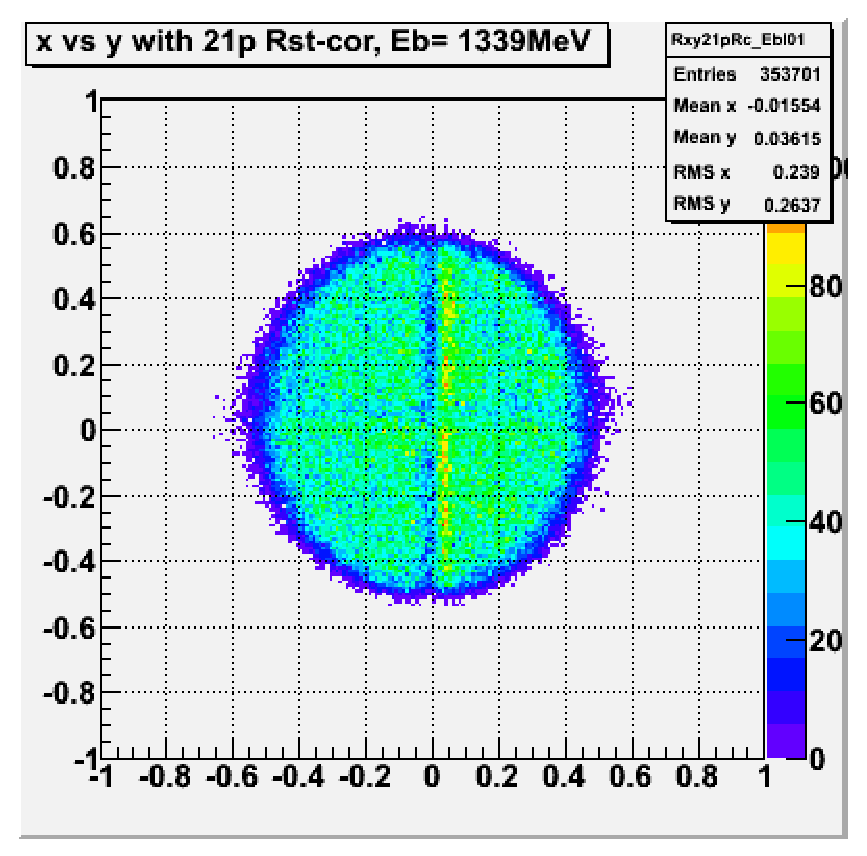
\epsfig{height=10cm,width=10cm,file=figuresEG4/FigKineCor/Rst21pCorXY.png}}  %kp: Disabled for Suman Jee's trimming test (enable back)
%\centerline{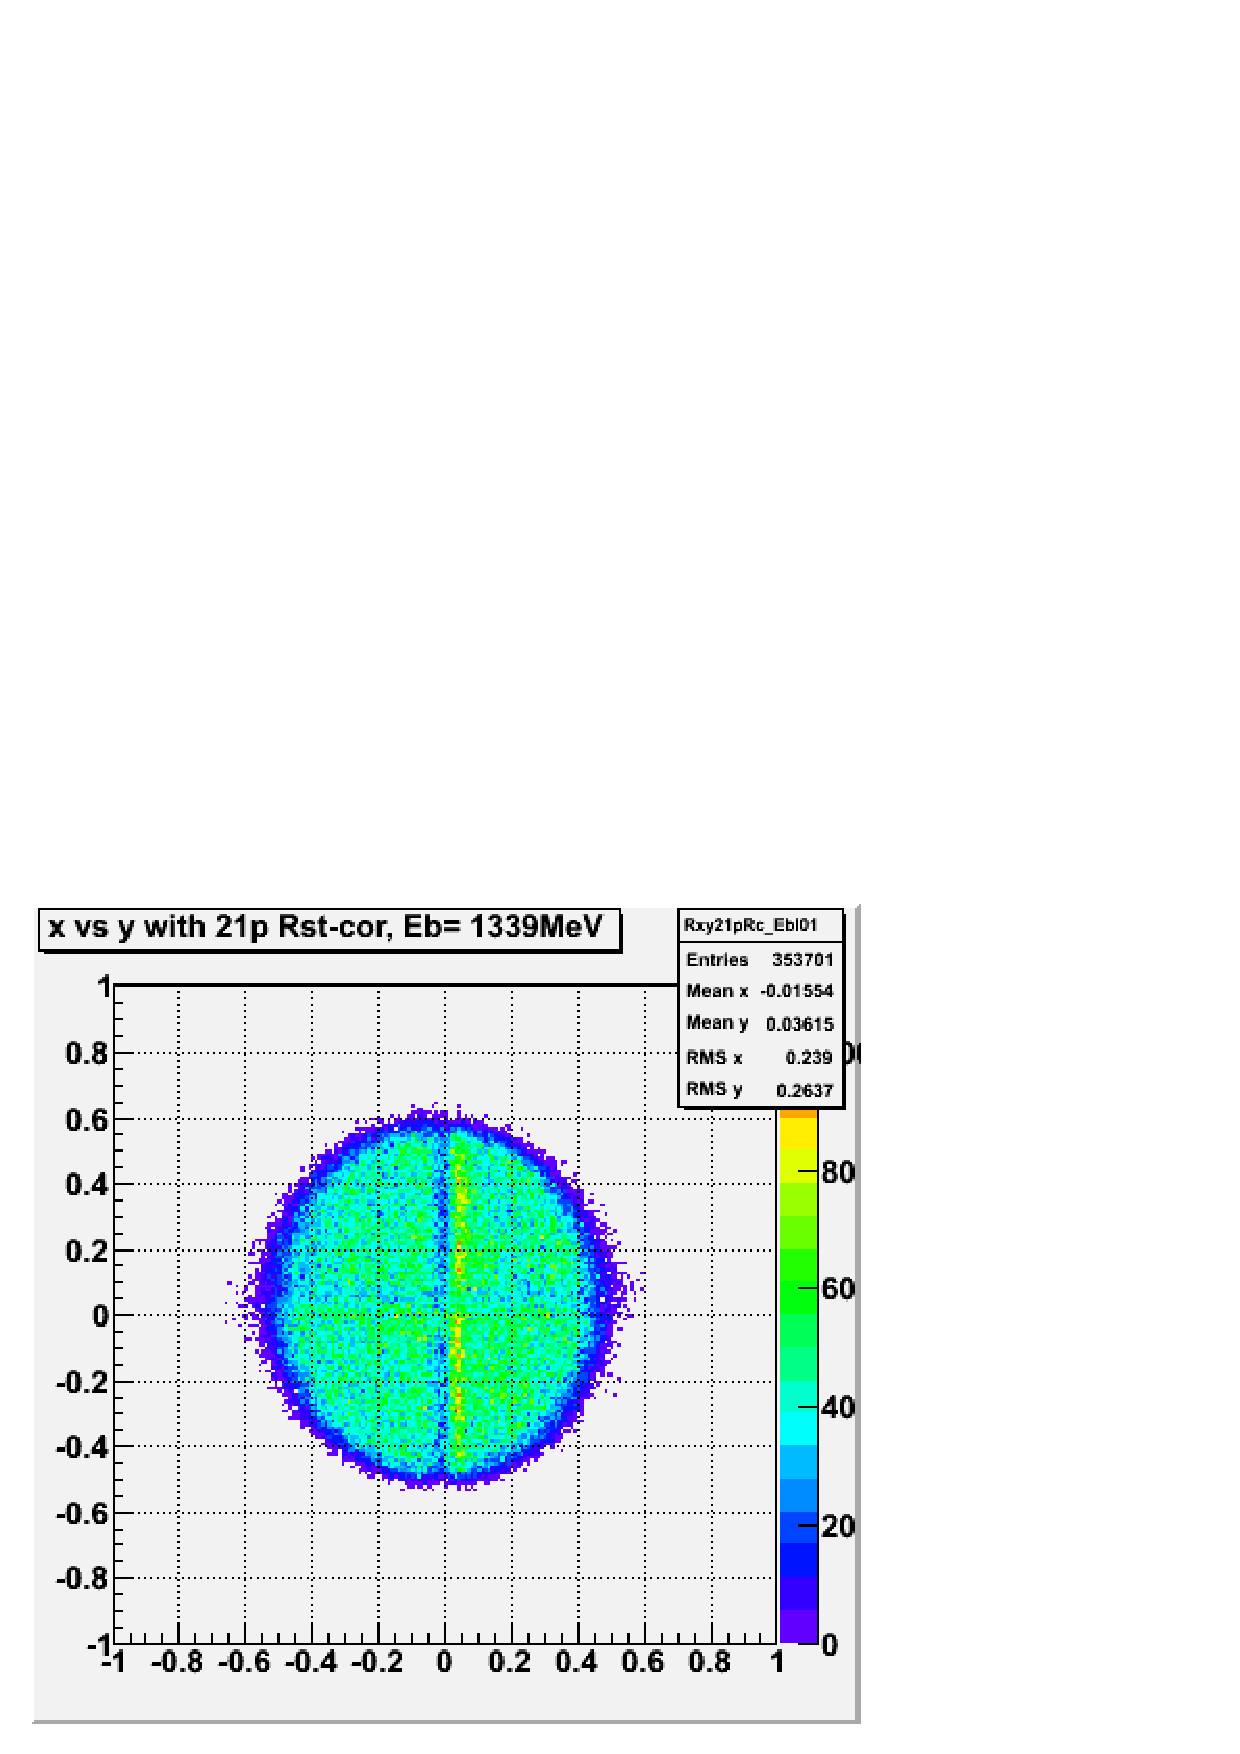
\includegraphics[trim = 0mm 0mm 0mm 50mm, clip = true, scale = 0.5] {chap7KineCor/figures/Rst21pCorXY.png}} %7/27/12
\caption{Beam coordinates x and y calculated with the raster correction procedure.}
\label{fig:RstXY}
\end{figure}

The procedure assumes that a linear relation holds between the raster currents and the beam coordinates x and y (displacements %bendings 
in cm produced by the field of the currents) as follows:

\begin{subequations}
\label{eqRC-Adc2cm}
\begin{eqnarray}
\label{eqRC-Adc2cm1}
x = (X_{adc}-X_{offset})C_x,
\end{eqnarray}

\begin{eqnarray}
\label{eqRC-Adc2cm2}
y = (Y_{adc}-Y_{offset})C_y,
\end{eqnarray}
\end{subequations}
where, $X_{offset}$, $Y_{offset}$, $C_x$, and $C_y$ are the %constants/
parameters to be determined by the procedure. These parameters are determined by selecting reasonably well reconstructed events each consisting of more than one charged  particles tracks originating reasonably close to the nominal target center (v$_z \approx $- 101.0 cm) and using them in TMinuit (ROOT Minuit program) to minimize the $\chi^2$, defined as
\begin{eqnarray}
\label{eqRC-chiSq}
\chi^2 = \sum^N_{i=1}((z_{corr})_i - z_o)^2,
\end{eqnarray}
where $z_0$ is the 5th parameter that defines the center of the target and is to be determined from the minimization. %/fitting. 
Likewise, $z_{corr}$ is the trial value of the corrected z-vertex (a function of trial values of the first four fit parameters, as will be evident below). TMinuit will give us those values of the parameters which gives 
the $\chi^2$ a minimum value.

\begin{comment}
\begin{figure}[h] %ht, htpb (p - float, b = bottom, h=? t = top)
\centerline{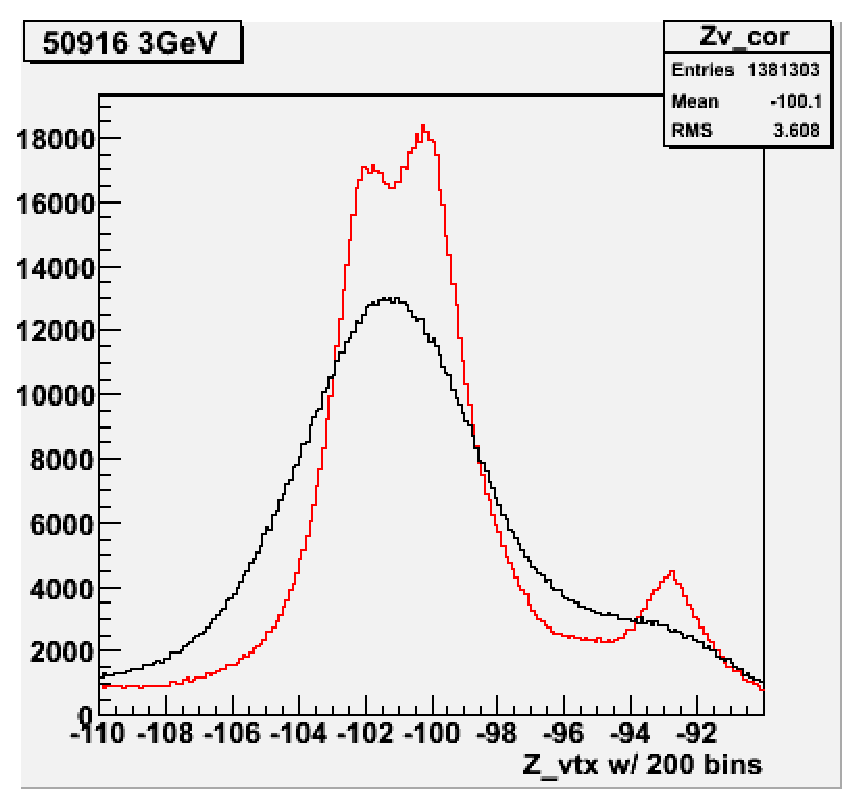
\epsfig{height=15cm,width=15cm,file=figuresEG4/FigKineCor/MTc3G50916one.png}}
\caption[Vz from Empty target run]{Vertex Z-coordinates of scattered electrons from an 3.0 GeV empty-cell-target run}
\label{fig:MTcellVz1}
\end{figure}
\end{comment}

\begin{figure}[h] 
\centering
  \leavevmode 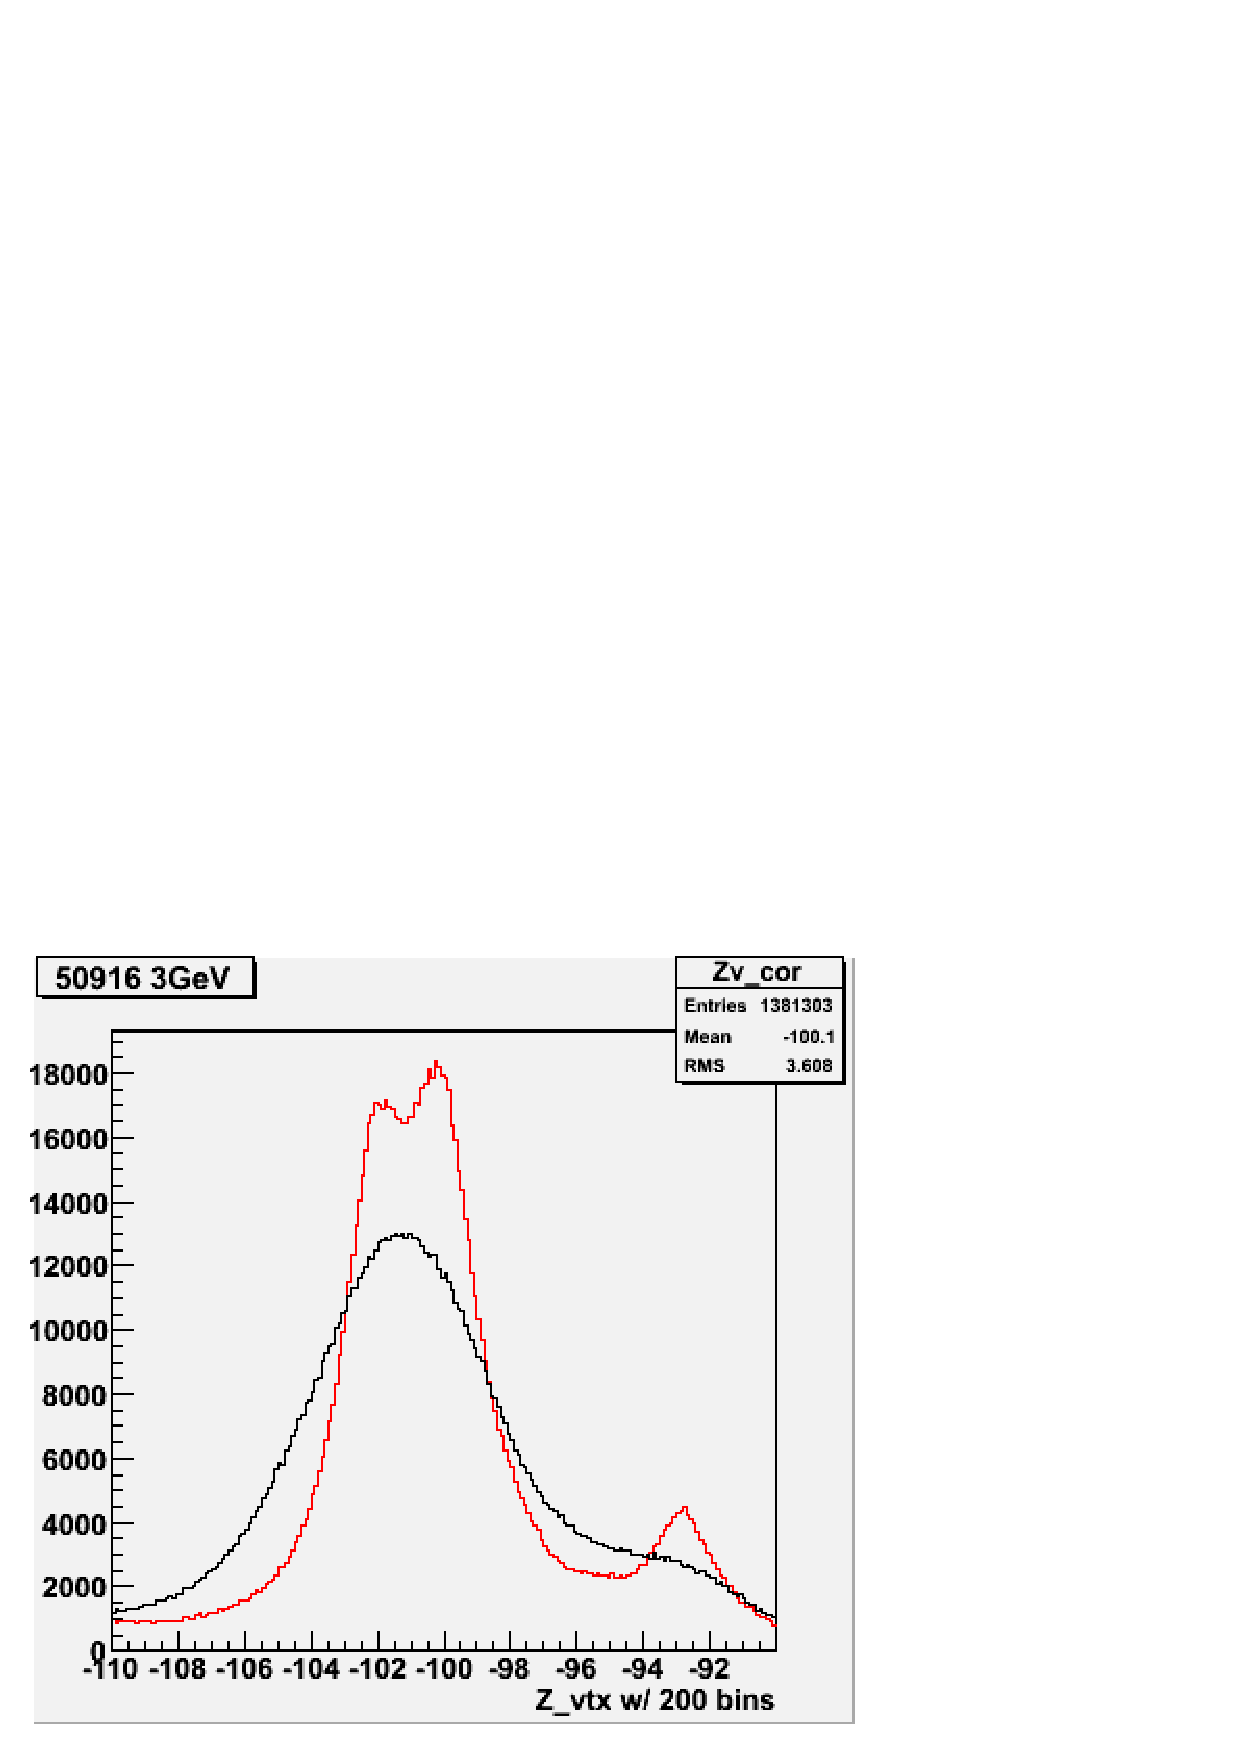
\includegraphics[width=0.8\textwidth]{figuresEG4/FigKineCor/MTc3G50916one.png}   
  \caption[Vz from Empty target run]{Vertex Z-coordinates (in cm) of scattered electrons from an 3.0 GeV empty-cell-target run before (black) and after (red) the raster corrections. It is clear that the correction improves the resolution, thus revealing the positions of the empty target cells (the first two peaks near -101.0 cm) and the heat shield (around -93.0 cm).}
  \label{fig:MTcellVz1}
\end{figure}



From a simple geometry consideration (as illustrated in Figs. \ref{fig:RstGeoKuhn1} and \ref{fig:RstGeoKuhn2}), an expression for correction to the z-vertex in terms of x, y and angles of a particle track is arrived at as follows:
\begin{eqnarray}
\label{eqRC-zcor}
z_{corr} = z_{recsis} + x'/tan(\theta),
\end{eqnarray}
where $z_{recsis}$, and $z_{corr}$ are the z-vertex measured %/reconstructed 
by the tracking code and the raster-corrected z-vertex respectively, and
\begin{eqnarray}
\label{eqRC-xprime}
x' = (x~cos\phi_s + y~sin\phi_s)/cos(\phi - \phi_s),
\end{eqnarray}
is the distance in cm along the track length that was not considered in tracking (because the tracking code assumes that the track started from $x = 0$, $y = 0$); $\phi_s$ is the sector angle defined as the azimuthal angle of the sector mid-plane (equal to $(s-1 \cdot 60$ degrees, where $s$ is the sector number from 1 to 6), and $\phi$ is the azimuthal angle of the particle (in the lab-coordinate system) defined as $\phi = arctan(cy/cx)$, %atan2(cy,cx), atan2 is a programming jargon, just write "arctan" %SEK
where $cx$ and $cy$ are the x- and y- direction cosines of the track. 

Due to the difference of the actual track length (through the 50 kG magnetic field of the target) from what is assumed by the tracking software, the azimuthal angle \phs is reconstructed incorrectly. The angle \phs can now be corrected by adding a correction term $- 50 q (x'/100)/33.356/p_t$ to the reconstructed value $\phi_{recsis}$ as follows:
\begin{eqnarray}
\label{eqRC-phcor}
\phi_{corr} = \phi_{recsis} - 50 q (x'/100)/33.356/p_t,
\end{eqnarray}
where $\phi_{recsis}$ and $\phi_{corr}$ are the reconstructed and corrected values of \phs respectively, $q$ is the particle charge in units of $e$, the factor 50 is the target field expressed in kG, the factor 100 is to convert the unit cm of $x'$ to m, the factor 33.356 is the inverse speed of light in the appropriate units and $p_t=p sin(\theta)$ is the particle's transverse momentum expressed in GeV \cite{rstcor_cn}.

% =====   12/5/13
For our analysis, all the four parameters $X_{offset}$, $Y_{offset}$, $C_x$, and $C_y$ were determined separately for each beam energy by selecting a set of good electrons and using the method of $\chi^2$ minimization (see Eq. \ref{eqRC-chiSq}). With the parameters known, we can use Eqs. \ref{eqRC-Adc2cm1} and \ref{eqRC-Adc2cm} to convert the X- and Y- ADC values into beam positions (at the target location) in centimeters as shown in Fig. \ref{fig:RstXY} for 1.3 GeV data. Likewise,  $vz$ and \phs can be corrected by calculating the correction terms $x'/tan(\theta)$ and $- 50 q (x'/100)/33.356/p_t$ and adding them to the respective reconstructed values (see Eqs. \ref{eqRC-zcor}, \ref{eqRC-phcor}). For example, Fig. \ref{fig:MTcellVz1} shows the distribution of electron Z-vertex distribution (from 3 GeV proton data) before and after the corrections. It is evident from the figure that the corrections improves the resolution as expected in addition to shifting (towards left) the average position of the distribution by some amount.
%\textcolor{red}{SEK: Section missing: What is the actual correction on Z, \ph? also, comment on result of fit procedure Fig. \ref{fig:RstXY}, and how it is applied to Zcor. }

%\input{trackingCorrectionsEG4.tex}
%% LyX 2.1.1 created this file.  For more info, see http://www.lyx.org/.
%% Do not edit unless you really know what you are doing.
%%kp: \documentclass[english]{article}
%%kp: \usepackage[T1]{fontenc}
%%kp: \usepackage[latin9]{inputenc}
%%kp: \usepackage{babel}
%%kp: \usepackage{latexsym}
%%kp: \usepackage{amstext}
%%kp: \usepackage{graphicx}
%%kp: \usepackage[unicode=true]
%%kp:  {hyperref}

%%kp: \makeatletter
%%kp: \AtBeginDocument{
%%kp:   \def\labelitemiii{\(\rhd\)}
%%kp:   \def\labelitemiv{\(\oplus\)}
%%kp: }
%%kp: 
%%kp: \makeatother
%%kp: 
%%kp: \begin{document}

%%kp: \title{Tracking Corrections}
%\section{Tracking Corrections}
\subsection{Tracking Corrections}
%%kp: 
%%kp: \maketitle
%%kp: 
%%kp: \section{Introduction}

This work is mostly based on the work documented in the \href{https://www.jlab.org/Hall-B/secure/eg1-dvcs/technotes/targetinfo/target_info.pdf}%{EG1-DVCS technical note \#{} 4}
{EG1-DVCS-TN-004}\cite{trkCorNote} %xz: you can be consistent and say this as you do below.
%by P. Bosted
, in which a routine or method is developed
to swim the particles through the field map of the target magnet to
the drift chambers in order to determine the particle angles and position
at the target, provided the direction cosines of the tracks at DC
and the beam position from the raster magnets are known. It is expected
that the method improves both the angular resolution and the reconstructed
logitudinal vertex position. The slightly modified version of the
corresponding C/C++ routine is used with some of the constants in
the routine replaced by new parameters to be determined by the method
of \textbf{$\chi^{2}$-square minimization} using ep-elastic events.
%(We tried to find $e^{+}e^{-}$ pairs in our data set to use in the minimization just like in the EG1DVCS, but due to various reasons, we were unable to find them, and, therefore, had to settle with the ep-elastic events only).
(Since this data set didn't have enough $e^{+}e^{-}$ pairs, we didn't use them in the minimization like in the EG1DVCS.) %xz: "due to various reasons" What reasons?  SHould explain. If unknown, say unknown.


%\subsection{Method}
\subsubsection{Method}

First of all, in order to convert raster magnet ADCs into corresponding beam positions x0 and y0,
we need conversion parameters. These parameters are determined by using a method outlined in
\href{https://www.jlab.org/Hall-B/secure/eg1-dvcs/technotes/raster/raster.pdf}{EG1-DVCS-TN-002}\cite{rastXYnZ}% by P. Bosted and A. Kim.
. The method determines the values of the slopes and offsets that convert the X- and Y-raster ADC readings to 
corresponding beam positions x0 and y0 in cm by minimizing the sensitivity of target vertex position (vz) 
for charged tracks to beam motion. 


Next, ep-elastic events are skimmed (from all of the \textbf{$NH_{3}$}
target data-set) using electron ID cuts for the electrons (see section \ref{allCuts}) in the sixth sector and proton ID consisting mainly of the time-of-flight cuts are used to select protons in the third sector (opposite to the sixth one). Then missing momentum cuts (less than 0.1 GeV for each of the four components Px, Py, Pz and E) based on 4-momentum conservation requirements (within measurement uncertainties) are used to help further clean up the accidental coincidences. These skimmed events are saved in root files and later reused for the minimization process described here.


The cuts used in the initial data skimming required that each of the four missing components $(Px, Py, Pz, E)_{miss}$ be less than 0.1 GeV.

After that a correction routine involving a set of correction
equations with several unknown parameters are established. Then
with the help of TMinuit (ROOT version of Minuit), several sets of
trial values are given to these unknown parameters and the corresponding
correction is applied to the particles in the skimmed events. For
each set of these trial values, a specifically defined \textbf{$\chi^{2}$
}(see below) is evaluated looping over all the skimmed events and
the Minuit tries to find the optimum set of these parameter values
for which the \textbf{$\chi^{2}$} is minimum. Such an optimal
set of values are chosen as the correct values of these parameters
and is used in the eventual correction routine.


%\subsection{The correction routine}
\subsubsection{The correction routine}

The routine uses 17 constants (free parameters determined by the above mentioned process
of $\chi^{2}$-minimization) and the following input and output variables:
\begin{itemize}
\item \textbf{Input variables:} $x_{r}$, $y_{r}$, cxdc, cydc, xdc, ydc,
zdc, p, q. 

\begin{itemize}
\item $x_{r,}$, $y_{r}$ are x \& y beam positions as returned by the raster
correction routine (see appendix)
\item \textbf{cxdc, cydc} are direction cosines of the track as measured
at DC1
\item \textbf{xdc, ydc, zdc} are the coordinates of the track meausred at
DC1
\item p, q are the momentum and charge of the track
\end{itemize}
\item \textbf{Output variables:} cxc, cyc, czc, vzc (all three corrected
direction cosines and the corrected Z-coordinate at the vertex) .
\end{itemize}
The sequence of calculation steps taken (inside the routine) to arrive
at the output results are as follows (where, I am also using the notations
of P. Bosted i.e., subscripts '0' used to indicate variables at vertex,
subscript 'f' for those at the drift chambers (these are the tl1\_
variables in the ntuples), and the values of (x, y, z) are in cm):
\begin{itemize}
\item First of all, get ready the following constants and variables:

\begin{itemize}
\item \textbf{$f_{c}=\frac{B}{50}=0.995$} is the overall field correction 

\begin{itemize}
\item (i.e., the $B.dl$ correction factor. Our $B=4.97T$, with B in kG
$f_{c}$ is 0.995)
\end{itemize}
\item $targsign=1$
\item $\theta_{f}=acos(cz_{dc})$
\item $\phi_{f}=atan2(cy_{dc},cx_{dc})$
\end{itemize}
\item Then, $\theta_{f}$ is corrected (for the misalignment of the DC) as follows:

\begin{itemize}
\item If it's the electron in the event,

\begin{itemize}
\item $\theta_{f}=\theta_{f}+(\mathbf{par[0]}+\mathbf{par[1]}\times\phi_{f})\thinspace\frac{cos\theta_{f}}{cos\phi_{f}}+(\mathbf{par[2]}+\mathbf{par[3]}\times\phi_{f})\thinspace \sin\theta_{f}$
\end{itemize}
\item else if its the proton, 

\begin{itemize}
\item $\theta_{f}=\theta_{f}+(\mathbf{par[4]}+\mathbf{par[5]}\times\phi_{f})$ \\

\end{itemize}
\end{itemize}
\item Next, get $\phi_{0}$ without raster corrections yet %(this accounts for the misalignment of the DC).

\begin{itemize}
\item $\phi_{0}=\phi_{f}+targsign\times f_{c}\thinspace(0.186+\mathbf{par[10]}+(0.045+\mathbf{par[11]})\thinspace\theta^{2}+(0.008+\mathbf{par[12]})\thinspace\theta_{f}^{3}+(0.0032+\mathbf{par[13]})\thinspace\theta_{f}^{3}/p^{2})\thinspace\frac{q}{p}$
\end{itemize}
\item Correction to polar angle from focusing effect. First, get focusing
term for beam (x,y)=0. 

\begin{itemize}
\item $\delta\theta=f_{c}\thinspace(0.90\thinspace\theta_{f}+1.2\thinspace\theta_{f}^{3})/(100\thinspace p^{2})$
\end{itemize}
\item Displacement of beam along trajectory ($x_{p}$) and perpendicular
to it ($y_{p}$) 

\begin{itemize}
\item $x_{p}=x_{r}\thinspace cos\phi_{0}+y_{r}\thinspace \sin\phi_{0}$ 
\item $y_{p}=-(x_{r}+\mathbf{par[6]})\thinspace \sin\phi_{0}+(y_{r}+\mathbf{par[7]})\thinspace cos\phi_{0}$ 
\end{itemize}
\item Correction to $\delta\theta$ from radial target field, which only
depends on raster x and y but not vertex z. Also, no effect on peak
at zero! 

\begin{itemize}
\item $\delta\theta=\delta\theta\thinspace(1.+targsign\thinspace q\thinspace p\thinspace(0.5/\theta_{f})\thinspace(y_{p}/0.75))$
\end{itemize}
\item Now can get cz 

\begin{itemize}
\item $\theta_{0}=\theta_{f}+\delta\theta$
\item $cz_{c}=cos\theta_{0}$
\end{itemize}
\item Now $\phi_{0}$ again, this time including raster correction 

\begin{itemize}
\item $\phi_{0}=\phi_{f}+targsign\thinspace f_{c}\thinspace(0.186+\mathbf{par[10]}+(0.045+\mathbf{par[11]})\thinspace\theta^{2}+(0.008+\mathbf{par[12]})\thinspace\theta_{f}^{3}+(0.0032+\mathbf{par[13]})\thinspace\theta_{f}^{3}/p^{2})\thinspace\frac{q}{p}\thinspace(1-(0.09+\mathbf{par[14]})\thinspace\frac{0.35-\mathbf{par[15]}}{\theta_{f}}\thinspace x_{p})$
\end{itemize}
\item Get cx and cy using this cz 

\begin{itemize}
\item $cx_{c}=\sin\theta_{0}\thinspace cos\phi_{0}$
\item $cy_{c}=\sin\theta_{0\thinspace}\sin\phi_{0}$
\end{itemize}
\item Renomalize czc 

\begin{itemize}
\item $cz_{c}=\sqrt{1.0-cx{}_{c}^{2}-cy{}_{c}^{2}}$
\end{itemize}
\item \textbf{Apply target field rotation correction} 

\begin{itemize}
\item $cx_{c}=cx_{c}-targsign\thinspace q\thinspace\mathbf{par[8]}\thinspace cz_{c}/p$
\item $cy{}_{c}=cy_{c}+targsign\thinspace q\thinspace\mathbf{par[9]}\thinspace cz_{c}/p$
\end{itemize}
\item \textbf{Renormalize again:}

\begin{itemize}
\item $czc=\sqrt{1.0-cx{}_{c}^{2}-cy{}_{c}^{2}}$
\item $\theta_{0}=acos(cz_{c})$ 
\end{itemize}
\item \textbf{Get vertex z in cm} 

\begin{itemize}
\item $r_{dc}=\sqrt{(x_{dc}-x_{r})^{2}+(y_{dc}-y_{r})^{2}}$
\item $Z_{c}=Z_{dc}-\frac{r_{dc}-(22+\mathbf{par[16]})\thinspace cos\theta_{0\thinspace}(tan\theta_{0}-tan\theta_{f})}{tan\theta_{f}}$
\end{itemize}
\item Finally, the routine outputs (returns) the four corrected quantities

\begin{itemize}
\item \textbf{$cx_{c},cy_{c},cz_{c},Z_{c}$.}
\end{itemize}
\end{itemize}




%\subsection{Calculation of $\chi^{2}$ (to be minimized) }
\subsubsection{Calculation of $\chi^{2}$ (to be minimized) }

The chi-square has different components as follows:

$\mathbf{\chi^{2}=\chi_{Zvar}^{2}(e)+\chi_{Zvar}^{2}(p)+\chi_{Evar}^{2}+\chi_{miss}^{2}+\chi_{Ppen}^{2}+\chi_{Epen}^{2}+\chi_{Zpen}^{2}+\chi_{\Delta E}^{2}}$

where, 
\begin{itemize}
\item $\mathbf{\chi_{Zvar}^{2}(e)}$ and $\mathbf{\chi_{Zvar}^{2}(p)}$
are Z-variance contributions from electron and proton candidates in
the ep-elastic events and are calculated as $\mathbf{\chi}_{\mathbf{Zvar}}^{\mathbf{2}}=\frac{1}{N_{ep}-1}\Big(\sum Z_{c}^{2}-\frac{(\sum Z_{c})^{2}}{N_{ep}}\Big)/(0.05)^{2}$
separately for the electrons and protons. (Here, $Z_{c}$ is the corrected
$Z$ of vertex and $N_{ep}$ is the number ep-elastic events used
in the minimization)
\item $\mathbf{\chi}_{\mathbf{Evar}}^{\mathbf{2}}=\frac{1}{N_{ep}-1}\Big(\sum E_{b}^{2}-\frac{(\sum E_{b})^{2}}{N_{ep}}\Big)/(0.005)^{2}$
is $E_{b}$-variance contribution. (Here, $E_{b}=M_{p}\Big(\frac{1}{tan(\theta_{p})tan(\theta_{e}/2)}-1\Big)$
is the beam energy calculated after the angles are corrected by the
correction routine.)
\item $\mathbf{\chi}_{\mathbf{miss}}^{\mathbf{2}}=100\times\Big(\frac{\sum p_{x}^{2}(miss)+\sum p_{y}^{2}(miss)}{0.02^{2}}+\frac{\sum p_{z}^{2}(miss)+\sum E^{2}(miss)}{0.05^{2}}\Big)$
is missing four-momentum contribution. (Here, 100 is an arbitrary
number to make the weight of this contribution comparable to others.)
\item $\mathbf{\chi}_{\mathbf{Ppen}}^{\mathbf{2}}=\sum\limits _{i=0}^{16}\frac{(par[i]-iPar[i])^{2}}{0.01^{2}}$
is the contribution due to runawy penalty on free parameters of the
minimization. (Here, par{[}i{]} \& iPar{[}i{]} are the current and
initial values of the 'i'th parameter. In the first iteration, initial
values were set to either zeros or the corresponding values as determined
for EG1-DVCS by P. Bosted. In later iterations, they were set to the
values determined from the previous iteration of the minimization.)
\item $\mathbf{\chi}_{\mathbf{Zpen}}^{\mathbf{2}}=\sum\limits _{e,p}\Big(\sum\limits _{N_{ep}}\frac{(Z_{c}-(-100.93))^{2}}{0.05^{2}}\Big)$
is a penalty term when $Z_{c}$ runs away from the known/nominal target
center (-100.93 cm)
\item $\mathbf{\chi}_{\mathbf{Epen}}^{\mathbf{2}}=\sum\limits _{i=2}^{4}\Big(\frac{\sum\limits _{N_{ep}}E_{b}}{N_{ep}}-E_{0}\Big)^{2}/(0.005)^{2}$
is a pentalty term to constrain $E_{b}$ running away from the nominal
values $E_{0}$ of beam energy.
\item $\mathbf{\chi}_{\mathbf{\Delta E}}^{\mathbf{2}}=\Big(\sum\limits _{i=2}^{4}\frac{\sum\limits _{N_{ep}}(E_{b}-E_{0})^{2}}{N_{ep}}\Big)/(0.005)^{2}$
is another pentalty term to constrain $E_{b}$ running away from the
nominal values $E_{0}$ of beam energy.
\end{itemize}


%\subsection{Minimization }
\subsubsection{Minimization }

TMinuit is used to minimze the value of$\chi^{2}$ as calculated above
and, thereby, determine the values of the free parameters used in
the correction routine. The minimization was done in such a way that
the parameters were determined step by step - first deciding the first
six parameters (keeping others fixed to initial values), then next
two, then next two, then next four, then next 2 and finally the last
one respectively.


\subsubsection{Tracking Correction Results}

With the method of $\chi^{2}$-minimization described above, the following
set of values were determined for the 17 parameters from par{[}0{]}
through par{[}16{]} respectively:

-0.00165789, -0.00131314, -0.00643021, -0.00721441, -0.00775272, 0.00483673,
0.063387, -0.0615822, 0.00133127, 0.000839944, 0.0210091, -0.0363265,
0.00335536, 0.00104193, 2.51519, -0.0313527, -1.29325

As a result of the corrections with these newly determined parameter
values, various quantites before and after the corrections looked
as shown in the following figure:

%\begin{comment}
\begin{figure} [H]
%\includegraphics[scale=0.345]{Images/trkCorrPass2_ep}
\includegraphics[scale=0.345]{figuresEG4/FigKineCor/trkCorrPass2_ep}

\protect\caption{Comparing various quantities before and after the tracking corrections which affects only the angles (and not the magnitude 'p') of the momentum.}
\end{figure}








\begin{comment}
\subsection{Conclusion}

The new tracking correction routine for EG4 with our own values of
parameters (determined by the method of $\chi^{2}$-minimization using
ep-elastic events) gave just a little better result than the original
version of the routine that was developed by P. Bosted for EG1-DVCS
data.





\section{Appendix}


\subsection{Raster x \& y (in cm):}

Raster x and y (denoted as $x_{r}$ and $y_{r}$ in cms) come as output
from the \textbf{raster correction routine} that was developed during
the past EG4 (pass1) analysis. These are simply translations (into
centimeters) of raster ADC values as measured for the x and y arms
of the raster magnet system, and thus they represent the beam position
in the XY-plane located at the target position along the beam line.

The \textbf{raster correction routine} has 21 parameters deterimined
by a $\chi^{2}$- minimization process. 
\begin{verse}
Par{[}21{]} = \{3.42931e-05, 0.000422835, -4.07979e-05, -0.000420968,
4330.72, 4440.27, -101.022, 4129.42, 4340.07, -101.064, 4104.95, 4251.29,
-101.041, 4014.65, 3946.27, -101.052, 4192.43, 3343.59, -101.002,
0.00096982, 0.00201097\};
\end{verse}
It takes 9 variables as inputs:

$E_{i}$, q, $X_{ADC}$, $Y_{ADC}$, p, all three direction cosines
(cx, cy, cz) of the track and Z of the vertex.

(Here, Ei=0,1,2,3, \& 4 for 1.0, 1.3, 2.0, 2.3, \& 3.0 GeV data sets
respectively)
\begin{description}
\item [{And}] the routine returns four quantities: $x_{r}$, $y_{r}$,
corrected $\textrm{\ensuremath{\phi}}$ and corrected Z as outputs.
The calculations of the corrections are done as follows:\end{description}
\begin{itemize}
\item Calculate $\theta$ and $\phi$ at vertex using the direction cosines.
\item Calculate the sector angle ($\phi_{s}$) i.e. the $\phi$ of the sector
mid-plane (= $(Sector-1)\times60$.)
\item $Z_{cor}=Z+\frac{X_{p}}{tan(\theta)}+factor1\times factor2$ 
\item $\phi_{cor}=\phi-q\times50.0\times\frac{X_{p}}{100}\times\frac{1}{33.356\times P_{t}}$
where

\begin{itemize}
\item $X_{gain}=Par[0]+\frac{Par[1]}{E_{b}}$
\item $Y_{gain}=Par[2]+\frac{Par[3]}{E_{b}}$
\item $X_{offset}=Par[3\thinspace E{}_{i}+4]$
\item $Y_{offset}=Par[3\thinspace E{}_{i}+5]$
\item $x_{r}=(X_{ADC}-X_{offset})\thinspace X_{gain}$
\item $y_{r}=(Y_{ADC}-Y_{offset})\thinspace Y_{gain}$
\item $X_{p}=(x_{r}\thinspace \cos\phi_{s}+y_{r}\thinspace \sin\phi_{s})/\cos(\phi-\phi_{s})$
\item $factor1=q\cdot10\cdot(Par[19]\cdot cx+Par[20]\cdot cy)\frac{1}{p\times \sin\theta\times \sin\theta}$; 
\item $factor2=\frac{1-0.25\times tan\theta\times tan\theta}{\sin\theta\times \cos\theta}$ 
\item $P_{t}=p\times \sin\theta$
\end{itemize}
\end{itemize}
\begin{thebibliography}{1}
\bibitem[1]{key-1}Tracking from Drift Chambers to Target through
Solenoid (\href{https://www.jlab.org/Hall-B/secure/eg1-dvcs/technotes/targetinfo/target_info.pdf}{EG1-DVCS Techical Note \#{} 004}),
P. Bosted

\bibitem[2]{key-2} Raster Corrections, P. Bosted, S. Kuhn \& Y. Prok.
CLAS-NOTE-03-008.

\bibitem[3]{key-3}Momentum Corrections for E6, A. Klimenko \& S.
Kuhn. CLAS-NOTE-03-005.\end{thebibliography}

\end{document}

\end{comment}

%%\textcolor{red}{KPA: Based on your comments on ``thesisV1\_edit'', I think, I will have to invest quite a lot of time on this section in reorganizing as well as explaining. So, I decided not to do anything substantial for now (before the defense) other than a few fixes of ``typo''. \\  \\ SEK: I agree. Skip this part for now. }

%\subsection{Overview}
\subsection{Drift Chamber (DC) Dependent Momentum Correction} 
%\subsubsection{Drift Chamber Dependent Correction Momentum Correction} %No subsection number shows up
%\subsubsubsection{Drift Chamber Dependent Correction Momentum Correction} //Didn't work

Different DC related factors contribute to the biggest part of the systematic deviations of particle momenta as reconstructed by RECSIS. The drift chambers could be misaligned relative to their nominal positions or the survey results that is used by RECSIS could be inaccurate or out-of-date. The effects of physical deformations (due to thermal and stress distortions) of the chamber including wire-sag, incorrect wire positions may not have bee incorporated properly. The torus field map used by the reconstruction software may not have been accurate and complete enough \cite{e6momcor_cn}. To address issues like these, a general approach as described in \cite{e6momcor_cn} which makes corrections to $p$ and \ths was followed to develop the corrections.

%SEK comment 12/4/13: The ordering of this still seems backward - FIRST explain the general scheme (corrections for p AND theta based on 4-momentum conservation, THEN explain that for sector 6 (and therefore electrons) we only use the momentum correction part

Particles detected in the 6th sector were treated differently than the others. (Reason to be elaborated later on). The DC dependent momentum correction was developed for the sixth sector and other sectors separately and with different methods. Since, there was sufficiently large amount of data that came from the 6th sector, a straight forward approach of binning the scattered electron data in various kinematic bins, finding in them the momentum offsets and then using the offsets (in combination with an approximation of ionization energy loss correction) for a fit (to a parameterized function) was used to develop the correction function. This method provided correction to the magnitude p of the 3-momentum of a particle detected in the 6th sector. Because of various constraints, angular corrections were not easy to address and so left undone.
%\subsubsection{For Sector 6:}
%\paragraph{For Sector 6:}

%Particles whose tracks were detected in the 6th sector drift chambers were subjected to only p-correction. 
The ratio of the correction to the magnitude of the momentum could be expressed as: 

\begin{eqnarray}
\label{eqPCor}
\frac{\Delta p}{p} = Pcorr1 + Pcorr2 + PatchCorr
\end{eqnarray}
where,
\begin{eqnarray}
\label{eqPCor1}
%\frac{\Delta p}{p} = ((E+F\phi)\frac{\cos\theta}{\sin\phi} + (G+H\phi)\sin\theta)\frac{p}{qB_{torus}}  %Smallest normal sized parentheses
%\frac{\Delta p}{p} = \big( (E+F\phi)\frac{\cos\theta}{\sin\phi} + (G+H\phi)\sin\theta   \big) \frac{p}{qB_{torus}} % same as above
%\frac{\Delta p}{p} = \Big( (E+F\phi)\frac{\cos\theta}{\sin\phi} + (G+H\phi)\sin\theta   \Big) \frac{p}{qB_{torus}} %Bigger parentheses
%\frac{\Delta p}{p} = \bigg( (E+F\phi)\frac{\cos\theta}{\sin\phi} + (G+H\phi)\sin\theta   \bigg) \frac{p}{qB_{torus}} %Bigger parentheses
Pcorr1 = \left( (E+F\phi)\frac{\cos\theta}{\sin\phi} + (G+H\phi)\sin\theta   \right) \frac{p}{qB_{torus}} %Biggest parentheses
\end{eqnarray}


\begin{eqnarray}
\label{eqPCor2}
%\frac{\Delta p}{p} = (J \cos\theta + K \sin\theta) + (M \cos\theta+N \sin\theta)\phi
Pcorr2 = (J \cos\theta + K \sin\theta) + (M \cos\theta+N \sin\theta)\phi
\end{eqnarray}

\begin{eqnarray}
\label{eqPatchCor}
PatchCorr = 0.02\left(P + (Q + R\frac{\phi_{deg}}{30^\circ})(\frac{10^\circ}{\theta_{deg}})^3 \right) 
\end{eqnarray}


The quantity $B_{tor}$ stands for $\int{B_{\perp}dl}$ along the track length multiplied by the speed of light in the units 
of m/ns (c = 0.29979 m/ns) and is given by

\begin{eqnarray}
\label{eqBtor1}
%B_{tor} = 0.76 \frac{I_{tor}\sin^2(4\theta)}{3375\theta/rad} \quad  for \quad  \theta < \frac{\pi}{8} %itallic text 'for'
B_{tor} = 0.76 \frac{I_{tor}\sin^2(4\theta)}{3375\theta/rad} \quad  \rm{for} \quad  \theta < \frac{\pi}{8} %Roman (no itallic)
%B_{tor} = 0.76 \frac{I_{tor}\sin^2(4\theta)}{3375\theta/rad} \quad  \mathrm{for} \quad  \theta < \frac{\pi}{8} %Roman (no itallic)
%B_{tor} = 0.76 \frac{I_{tor}\sin^2(4\theta)}{3375\theta/rad} \quad  \textrm{for} \quad  \theta < \frac{\pi}{8} %Roman (no itallic)
\end{eqnarray}

\begin{eqnarray}
\label{eqBtor2}
B_{tor} = 0.76 \frac{I_{tor}}{3375\theta/rad}  \quad  \textrm{for}  \quad  \theta > \frac{\pi}{8}
\end{eqnarray}

In all these equations, sector number, $\theta$, $\phi$, $\theta_{deg}$, and $\phi_{deg}$ come from the angle information measured at DC1. The direction cosine variables tl1\_cx, tl1\_cy, tl1\_cz (from pass1 ntuples) are used to derive these quantities. C++ standard functions acos() and atan2() are used to evaluate $\theta$, $\phi$ (w.r.t the sector mid plane). %(One should take an extra care of the fact that the function atan2() gives the values of azimuthal angle $\phi$ between -$\pi$ to +$\pi$.) %SEK cor 12/4/13



All these total of eleven unknown parameters were determined separately by fitting above mentioned momentum offsets (in combination with ionization energy loss correction for electrons) to the correction function given by the Eq. \ref{eqPCor}.




%\subsubsection{For Other (1-5) Sectors:}
%\paragraph{For Other (1-5) Sectors:}

Unlike for sector-6, both p- and $\theta$ were subjected to correction if a given particle track was detected by the drift-chamber in any of the other 5 sectors. This time, the PatchCorr component was not considered in the expression (Eq. \ref{eqPCor}) for p-correction. On the other hand, following expression was used to parameterize the correction to the polar angle $\theta$.

%\begin{equation} %equation reference didn't work with this  
\begin{eqnarray}
\label{eqThCor}
\Delta\theta = (A+B\phi)\frac{\cos\theta}{\cos\phi} + (C+D\phi)\sin\theta
%\end{equation} 
\end{eqnarray}

A total of 12 (8 for p-correction and 4 for $\theta$ correction) parameters for each of these five sectors were determined (from a fit procedure to be described below) to account for the DC contribution to the corrections. 









%\subsubsection{Solenoid Axis Tilt Correction} 
\subsection{Solenoid Correction} 

If the axis of the target solenoid field is not aligned exactly along the beam line% (as supposed to)
, then the $\phi$ reconstruction is skewed. To correct for that, the following changes %corrections are to be 
are made to the reconstructed angles: 

\begin{subequations}
\label{eqTiltCor}
\begin{eqnarray}
\label{eqTiltCor1}
cx_{true} = cx_{ini} + a/p %\newline cx_{true} = cx_{ini} + b/p
\end{eqnarray}

\begin{eqnarray}
\label{eqTiltCor2}
cy_{true} = cy_{ini} + b/p
\end{eqnarray}
\end{subequations}
where $cx$ and $cy$ are the x- and y- direction cosines, $p$ is the particle momentum and a and b are the parameters to be determined by the fit (described in \ref{secMcProcedure}). %{pCorFit2}). 
It's clear that $cx$ and $cy$ and therefore $\phi = arctan(cy/cx)$ %$\phi = atan2(cy,cx)$ is corrected 
is changed by this part of the correction.





%\subsubsection{Solenoid Axis Offset Correction} 

The target field may also have an overall displacement or offset w.r.t the beam line and so the following correction to
the angles is used in addition to the other corrections:

\begin{subequations}
\label{eqOffsetCor}
\begin{eqnarray}
\label{eqOffsetCor1}
\phi_{true} = \phi_{ini} + qB_{solenoid}\frac{S \cos\phi_{ini} - T \sin\phi_{ini}}{p \sin\theta_{ini}}
\end{eqnarray}

\begin{eqnarray}
\label{eqOffsetCor2}
\theta_{true} = \theta_{ini} + qB_{solenoid} \frac{U \cos\phi_{ini} - V \sin\phi_{ini}}{p}
\end{eqnarray}
\end{subequations}

Here, S, T, U and V are the additional parameters to be determined by the method of \chisqs minimization (see Sec. \ref{secMcProcedure}) for the overall correction.








%\subsubsection{Additional Vertex-Z Correction}
%\label{ssecVzCor} %sec for section and ssec for subsection and so on

RECSIS evaluates the vertex assuming that it lies on the intersection of the track and the plane perpendicular to the 
sector mid-plane that contains the beam axis \cite{kuhnDvcs_wb}. So, RECSIS backtracks the DC-reconstructed particle track and finds the point where
the track meets this plane %the sector mid-plane 
to determine the vertex. As a consequence, %This consideration is made 
while doing the raster correction, we correct % which corrects 
Z in addition to  $\phi$. Since the track itself is subject to further corrections even after the raster correction,
the vertex should also be corrected further. The following expression is used to further correct the z-component of the vertex.
\begin{eqnarray}
\label{eqExVzCor}
z_{true} = z_{rst} + Y \frac{\theta - \theta_{ini}}{\sin^2\theta}
\end{eqnarray}
where $\theta_{ini}$ is the polar angle (in radians) at the start, $\theta$ is the one after all the previous corrections and 'Y' is the new fitting parameter to be determined whose physical meaning is the distance from the vertex to the first region of DC (about 150 cm) \cite{slava_th}.


















\subsection{Outgoing Ionization Loss Correction}
\label{ssecElossCor}
 
%    \sqrt[root]{arg} The \sqrt command produces the square root of its argument. The optional argument, root, determines what root 
%    to produce, i.e., the cube root of x+y  would be typed as  $\sqrt[3]{x+y}$
After all the previous corrections are made, the energy of each of the particles is calculated as $E = \sqrt{p^2 + m^2_{rest}}$ and a correction for ionization loss is added to it: $E_{cor} = E + \Delta E $ with $\Delta E = \frac{dE}{dX}\tau$ % $\Delta E = (\frac{\Delta E/\Delta X}{1000.0})gm$,
where the factor $\tau$ is the total effective mass thickness traversed by the particle and
\begin{subequations}
\begin{eqnarray}
\label{eqElossEl}
%\Delta E/ \Delta X = 2.8 ~MeV \quad \rm{for ~electrons}
dE/dX \approx 2.8 ~\rm{MeV/(g ~cm}^{-2}\rm{)} \quad \rm{for ~electrons}
\end{eqnarray}
and, for hadrons \cite{leo1994techniques}
\begin{eqnarray}
\label{eqElossHad}
%%%if( mass < 0.01) DEDX = 2.8;    else DEDX = 0.307 * ( 0.5 / Beta2 ) * ( log( 2. * 511000.0 * Beta2 * ( Gamma2 / 90. ) ) - Beta2 );
%%%\Delta E/ \Delta X = 0.307 (\frac{ 0.5}{ \beta^2}) \left( log\bigg( 2.0( 511000.0 \beta^2) (\frac{ \gamma^2}{ 90.0} ) \bigg) - \beta^2 \right);
%%%\Delta E/ \Delta X = 0.307 (\frac{ 0.5}{ \beta^2}) \left( ln\bigg( 2.0( 511000.0 \beta^2) (\frac{ \gamma^2}{ 90.0} ) \bigg) - \beta^2 \right) ~MeV ~\rm{for ~hadrons} 
%\Delta E/ \Delta X = 0.307 \times \frac{ 0.5}{ \beta^2} \left( ln\bigg( 2.0 \times 511.0 \frac{\beta^2 \gamma^2}{ 0.090} \bigg) - \beta^2 \right) ~MeV 
dE/dX \approx 0.307 \times \frac{ 0.5}{ \beta^2} \left( ln\bigg( 2.0 \times 511.0 \frac{\beta^2 \gamma^2}{ 0.090} \bigg) - \beta^2 \right) \rm{~MeV} 
\end{eqnarray}
\end{subequations}
which is an approximation of the Bethe-Block formula \cite{leo1994techniques}: % (Eq.(\ref{eqBetheBlock})).

\begin{eqnarray}
\label{eqBetheBlock}
-\frac{1}{\rho} \frac{dE}{dx} = 4\pi N_a r_e^2 m_e c^2 \frac{Z}{A} \frac{1}{\beta^2} \left( ln\bigg( \frac{2m_ec^2\gamma^2\beta^2}{I} \bigg) - \beta^2 \right) 
\end{eqnarray}
%And, the factor '$\tau$' is the total effective mass thickness traversed by the particle. 
This quantity is calculated as follows:
\begin{itemize}
\item $\tau = \tau_{\parallel}/\cos\theta$ \quad if $\theta <= \pi/4$
\item $\tau = \tau_{\parallel}/\cos(\pi/4)$ \quad if $\theta > \pi/4$    %SEK comment:  I don't understand. leave out! Why not \tau = r/\sin \theta    (anyway \theta > \pi/4 is never true!
\end{itemize}
where $\tau_{\parallel}$ is calculated as:
\begin{itemize}
\item $\tau_{\parallel} = \Delta z \times 0.6 + 0.4$ \quad if $\Delta z > 0.0 $ and $\Delta z < 1.0 $
\item $\tau_{\parallel} = 0.6 + 0.4$ \quad if $\Delta z \geq  1.0$
\item $\tau_{\parallel} = 0.4$ \quad if $\Delta z \leq  0.0$
%\item $\tau_{\parallel} = 0.75$ \quad if otherwise
\end{itemize}
with $\Delta z = z_{target\_center} - z_{ave} + L_{target}/2 = (-101.0$ cm $ - z_{ave} + 0.5)$ cm being the physical distance (along the target length) traveled by the particle through the polarized target material (e.g. the EG4ND$_3$ target has length 1.0 cm and is positioned at z = -101.0 cm). The factor 0.6 is the effective mass thickness of ND$_3$ (density of ND$_3$ ($\sim 1 ~g/cm^3$) %(e.g. one of the EG4 NH$_3$ (ND$_3$ too) target has length 1.0 cm and is positioned at z = -101.0 cm). The factor 0.6 is the effective mass thickness of NH$_3$ (density of NH$_3$ ($\sim 1 ~g/cm^3$) 
multiplied by the packing fraction which is roughly 0.6 \cite{rferschAnaNote},%\cite{rfersch_th},
whereas 0.4 is the sum of the mass thicknesses of He ($\sim 0.3$) and that of window foils ($\sim 0.1$) \cite{nGuler_th}. %In fact these numbers were for NH3 targets and were decided when our own values for PFs were not available which are now at about 0.7 (I believe, this won't make things much different, may be systematic study has to be done. 12/5/13)


% double zcenter    = -101.0; //-55.1;//#ignore
%  double \Delta z = zcenter - zave + 0.5;//#ignore
%  //kp:  \Delta z is the fraction of the distance the particle travelled i.e. \Delta z = (zave - zcenter + 0.5)/Lt  (Lt = target length = 1.0 for EG1B)
%  //     (denoted by delta_z in Nevzat's thesis), also in thesis, the order of zave -zcenter is wrong.
%  double E = sqrt(p*p + mass*mass);
%  double fbeta = p/E;  double Beta2 = fbeta * fbeta; double Gamma2 = 1.0 / ( 1.0 - Beta2 );  
    
%    if( ( \Delta z <= 1.0 ) && ( \Delta z >= 0.0 ) )  \tau = \Delta z * 0.6 + 0.4;
%    //kp: I think \tau is total effective mass thickness traversed by the particle
%    //    The factor 0.6 is effective mass thickness of NH$_3$ (density of NH$_3$ (about 1 g/cm^3) multiplied by the packing fraction which is 
%    //    roughly 0.6; See R. Fersch's thesis at page 215) and 0.4 is the sum of 0.3 and 0.1 where
%    //    0.4 is for mass thickness of He and 0.1 for that of window foils (see Nevzat's thesis, page 158)

%    else if( \Delta z >= 1.0 )  \tau = 0.6 + 0.4;
%    else if( \Delta z <= 0.0 )  \tau = 0.4;
%    else  \tau = 0.75;
%   //Ignore all above lines with '#ignore' and use '\tau = 0.75' for all cases for a reasonable approximation (Dr. Kuhn)
    
%    if( theta * rad2deg <= 45. ) \tau = \tau / \cos( theta );
%    else  \tau = \tau / \cos( 45. * deg2rad );

Using the ionization loss corrected energy and the rest mass of the particle, momentum is recalculated as $p_{cor} = \sqrt{E^2_{cor}-m^2}$ (where $m$ is the mass of the particle). Finally, this new p is used along with the previously corrected angles to evaluate the three cartesian components $p_x$, $p_y$ and $p_z$ of the momentum.




%This file has descriptions of mom. and (outgoing) energy-loss corrections.
% Check the pass2 mom. cor. routine with a link available at the following wiki page:
%      https://clasweb.jlab.org/rungroups/eg4/wiki/index.php/Momentum_Correction_(Pass2)
%  or at https://www.jlab.org/Hall-B//secure/eg4/adhikari/myHomeLinked/MyHm/LinkedFiles/momCorPass2.h


\subsection{Momentum Correction}
Different DC related factors contribute to the biggest part of the systematic deviations of particle momenta as reconstructed by RECSIS. The drift chambers could be misaligned relative to their nominal positions or the survey results that is used by RECSIS could be inaccurate or out-of-date. The effects of physical deformations (due to thermal and stress distortions) of the chamber including wire-sag, incorrect wire positions may not have been incorporated properly. The torus field map used by the reconstruction software may not have been accurate and complete enough \cite{e6momcor_cn}. Effects on angles \th and \ph due to these contributions are already factored in the tracking correction described earlier. However, a separate method is developed to correct for the effect on the magnitude $p$ of the momentum. This $p$-correction methods picks up and builds on some of the ideas outlined in the CLAS-NOTE 2003-005 \cite{e6momcor_cn}.

\subsubsection{Procedure to determine the first 11 parameters}
\label{pCorFit1}
The procedure involved dividing the covered kinematic space into a number of bins, finding in them the magnitude of shifts of the inclusive 
elastic peaks w.r.t. the expected position and use that to fit to a function to get an analytical expression for the correction. The 
following angular bins were used:
\begin{itemize}
\item Six $\theta_{dc1}$ bins: (0,8),(8,10),(10,12),(12,15),(15,20),(20,30) degrees
\item Five $\phi_{dc1}$ bins: (-10,-6),(-6,-2), (-2,2), (2,6), (6,10) degrees 
\end{itemize}
where the angles used are the ones measured at the first drift chamber and $\phi_{dc1}$ is measured w.r.t the sector mid-plane (thus the 
maximum range allowed is (-30.0,30.0)).
  
\begin{eqnarray}
\label{eqElasticEprime}
E'_{elastic} = \frac{E_{beam}}{1+\frac{2E_{beam}}{M_p}sin^2(\theta_e/2)}
\end{eqnarray}

%\textcolor{red}{To be expanded later on.}

In each of these kinematic bins, the quantity $\Delta E = E'_{elastic} - p$ (see Eq. \ref{eqElasticEprime}) is histogrammed for both NH$_3$ and $^{12}$C data separately. Next, the carbon histogram is cross-normalized with the ammonia histogram (by comparing the two in the region left to the quasi-elastic peak) and subtracted from the latter one to remove the nuclear background. The difference gives  histograms for the elastic events (as shown by the dashed green histogram in Fig. \ref{sec6dEall}). A Gaussian fit to the extracted elastic histogram gives the position and width of the distribution. The offset or shift of average position of the peak with respect to the expected $\Delta E = 0$ gives us the needed correction on energy $E \approx p$ for the electron. This process is repeated for all of the bins listed above and the corresponding $\Delta E$ offsets or the corrections are determined for each of them. Additionally, $\Delta E$ distributions using $^{15}N$ nuclear mass in calculating $E'_{elastic}$ are also made and off-sets in the corresponding elastic peaks are also recorded whenever possible (particularly from the lower \th bins from low beam energy data where the nuclear-elastic and quasi-elastic peaks are well separated).
% https://clasweb.jlab.org/rungroups/eg4/wiki/index.php/Momentum_Correction_(Pass2)#6.2F23-30.2F15
%https://www.jlab.org/Hall-B//secure/eg4/adhikari/Corrections/Mcor/Pass2/IncMcor/GfOp/elasticPeaksFromNH3wdWoCorEi0.gif
%https://www.jlab.org/Hall-B//secure/eg4/adhikari/Corrections/Mcor/Pass2/IncMcor/GfOp/elasticPeaksFromNH3wdWoCorEi0mN15.gif
Finally, these values of corrections for different average values of $\theta_{dc1}$ and $\phi_{dc1}$ are fit to Eq. \ref{eqPCor} (which is based on similar work done for EG1b analysis\cite{nGuler_th})
and using the method of \chisq-minimization in order to determine the values of the 11 fit parameters.


\begin{eqnarray}
\label{eqPCor}
\frac{\Delta p}{p} = Pcorr1 + Pcorr2 + PatchCorr
\end{eqnarray}
where, $\frac{\Delta p}{p}$ is the ratio of the correction ($\Delta p$) to the magnitude ($p$) of the momentum and 
\begin{eqnarray}
\label{eqPCor1}
%\frac{\Delta p}{p} = ((E+F\phi)\frac{cos\theta}{sin\phi} + (G+H\phi)sin\theta)\frac{p}{qB_{torus}}  %Smallest normal sized parentheses
%\frac{\Delta p}{p} = \big( (E+F\phi)\frac{cos\theta}{sin\phi} + (G+H\phi)sin\theta   \big) \frac{p}{qB_{torus}} % same as above
%\frac{\Delta p}{p} = \Big( (E+F\phi)\frac{cos\theta}{sin\phi} + (G+H\phi)sin\theta   \Big) \frac{p}{qB_{torus}} %Bigger parentheses
%\frac{\Delta p}{p} = \bigg( (E+F\phi)\frac{cos\theta}{sin\phi} + (G+H\phi)sin\theta   \bigg) \frac{p}{qB_{torus}} %Bigger parentheses
Pcorr1 = \left( (E+F\phi)\frac{cos\theta}{sin\phi} + (G+H\phi)sin\theta   \right) \frac{p}{qB_{torus}} %Biggest parentheses
\end{eqnarray}


\begin{eqnarray}
\label{eqPCor2}
%\frac{\Delta p}{p} = (J cos\theta + K sin\theta) + (M cos\theta+N sin\theta)\phi
Pcorr2 = (J cos\theta + K sin\theta) + (M cos\theta+N sin\theta)\phi
\end{eqnarray}

\begin{eqnarray}
\label{eqPatchCor}
PatchCorr = 0.02\left(P + (Q + R\frac{\phi_{deg}}{30^\circ})(\frac{10^\circ}{\theta_{deg}})^3 \right) 
\end{eqnarray}

The quantity $B_{tor}$ stands for $\int{B_{\perp}dl}$ along the track length multiplied by the speed of light in the units 
of m/ns (c = 0.29979 m/ns) and is given by

\begin{eqnarray}
\label{eqBtor1}
%B_{tor} = 0.76 \frac{I_{tor}sin^2(4\theta)}{3375\theta/rad} \quad  for \quad  \theta < \frac{\pi}{8} %itallic text 'for'
B_{tor} = 0.76 \frac{I_{tor}sin^2(4\theta)}{3375\theta/rad} \quad  \rm{for} \quad  \theta < \frac{\pi}{8} %Roman (no itallic)
%B_{tor} = 0.76 \frac{I_{tor}sin^2(4\theta)}{3375\theta/rad} \quad  \mathrm{for} \quad  \theta < \frac{\pi}{8} %Roman (no itallic)
%B_{tor} = 0.76 \frac{I_{tor}sin^2(4\theta)}{3375\theta/rad} \quad  \textrm{for} \quad  \theta < \frac{\pi}{8} %Roman (no itallic)
\end{eqnarray}

\begin{eqnarray}
\label{eqBtor2}
B_{tor} = 0.76 \frac{I_{tor}}{3375\theta/rad}  \quad  \textrm{for}  \quad  \theta > \frac{\pi}{8}
\end{eqnarray}

In all these equations, sector number, $\theta$, $\phi$, $\theta_{deg}$, and $\phi_{deg}$ come from the angle information measured at DC1. The direction cosine variables tl1\_cx, tl1\_cy, tl1\_cz (from pass1 ntuples) are used to derive these quantities. C++ standard functions acos() and atan2() are used to evaluate $\theta$, $\phi$ (w.r.t the sector mid plane). %(One should take an extra care of the fact that the function atan2() gives the values of azimuthal angle $\phi$ between -$\pi$ to +$\pi$.) %SEK cor 12/4/13



These total of eleven unknown parameters were determined by fitting above mentioned momentum offsets (in combination with ionization energy loss correction for electrons (see Sec.\ref{secElossCor} below)) to the correction function given by the Eq. \ref{eqPCor}.




\begin{figure}[H]%[ht] 
%\centerline{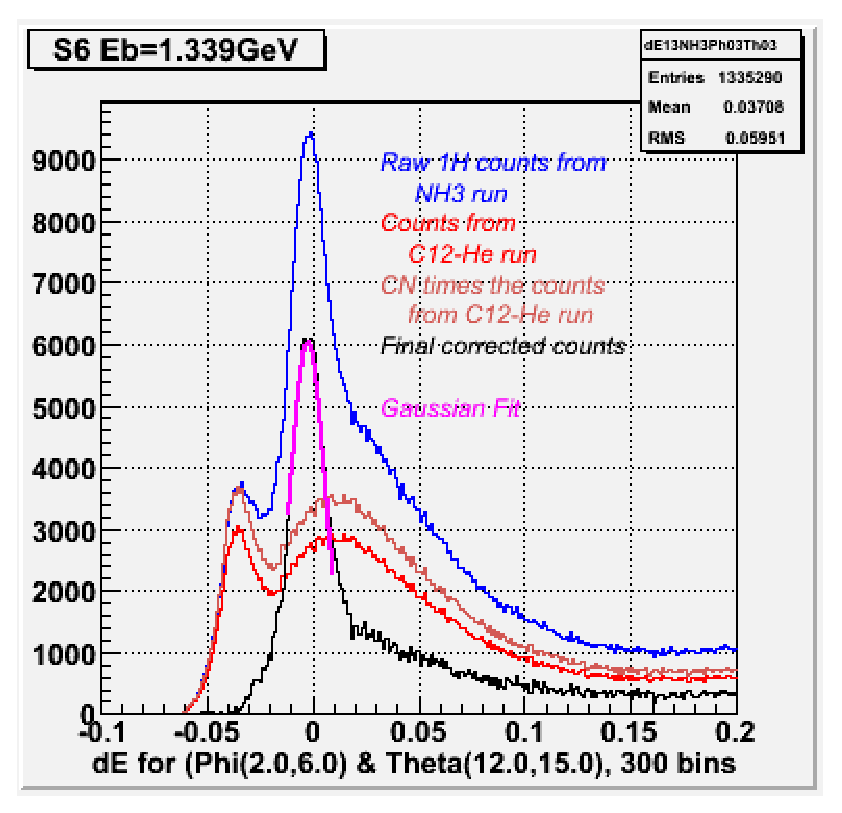
\epsfig{height=10cm,width=15cm,file=chap7KineCor/figures/HiStatNH3_1339_3_o1.eps}}
%\caption[The world data for the proton form factor ratio $\mu_p\frac{G_E}{G_M}$ extracted using Rosenbluth separations.]{The world 
%data for the proton form factor ratio $\mu_p\frac{G_E}{G_M}$ extracted using Rosenbluth separations ~\cite{qatan_th}.}
%\caption[Background removal from $\Delta E$]{Plot showing background removal from the $\Delta E$ counts (shown in blue) from $NH_3$ data 
%(by subtracting cross-normalized counts from $^{12}C$ data (shown in red)) to separate the elastic peak (black) in one of the kinematic bins, 
%thereby getting the momentum offset for that bin.}
\centering
  %\leavevmode 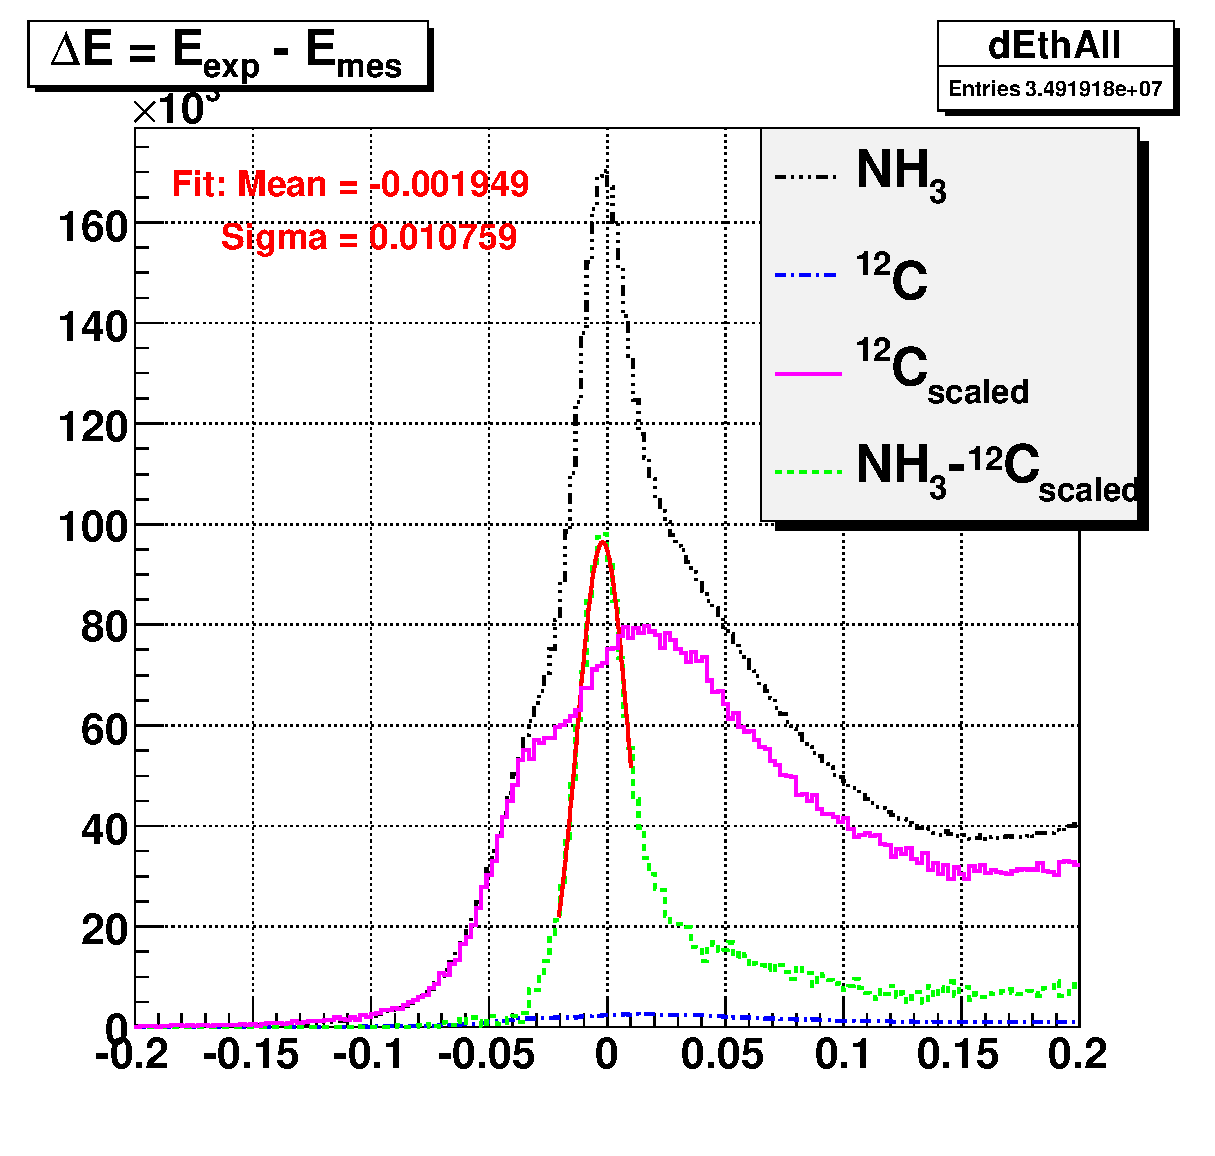
\includegraphics[width=0.8\textwidth]{chap4simul/DcSmear/dE_elastProdEb3.eps} 
  \leavevmode 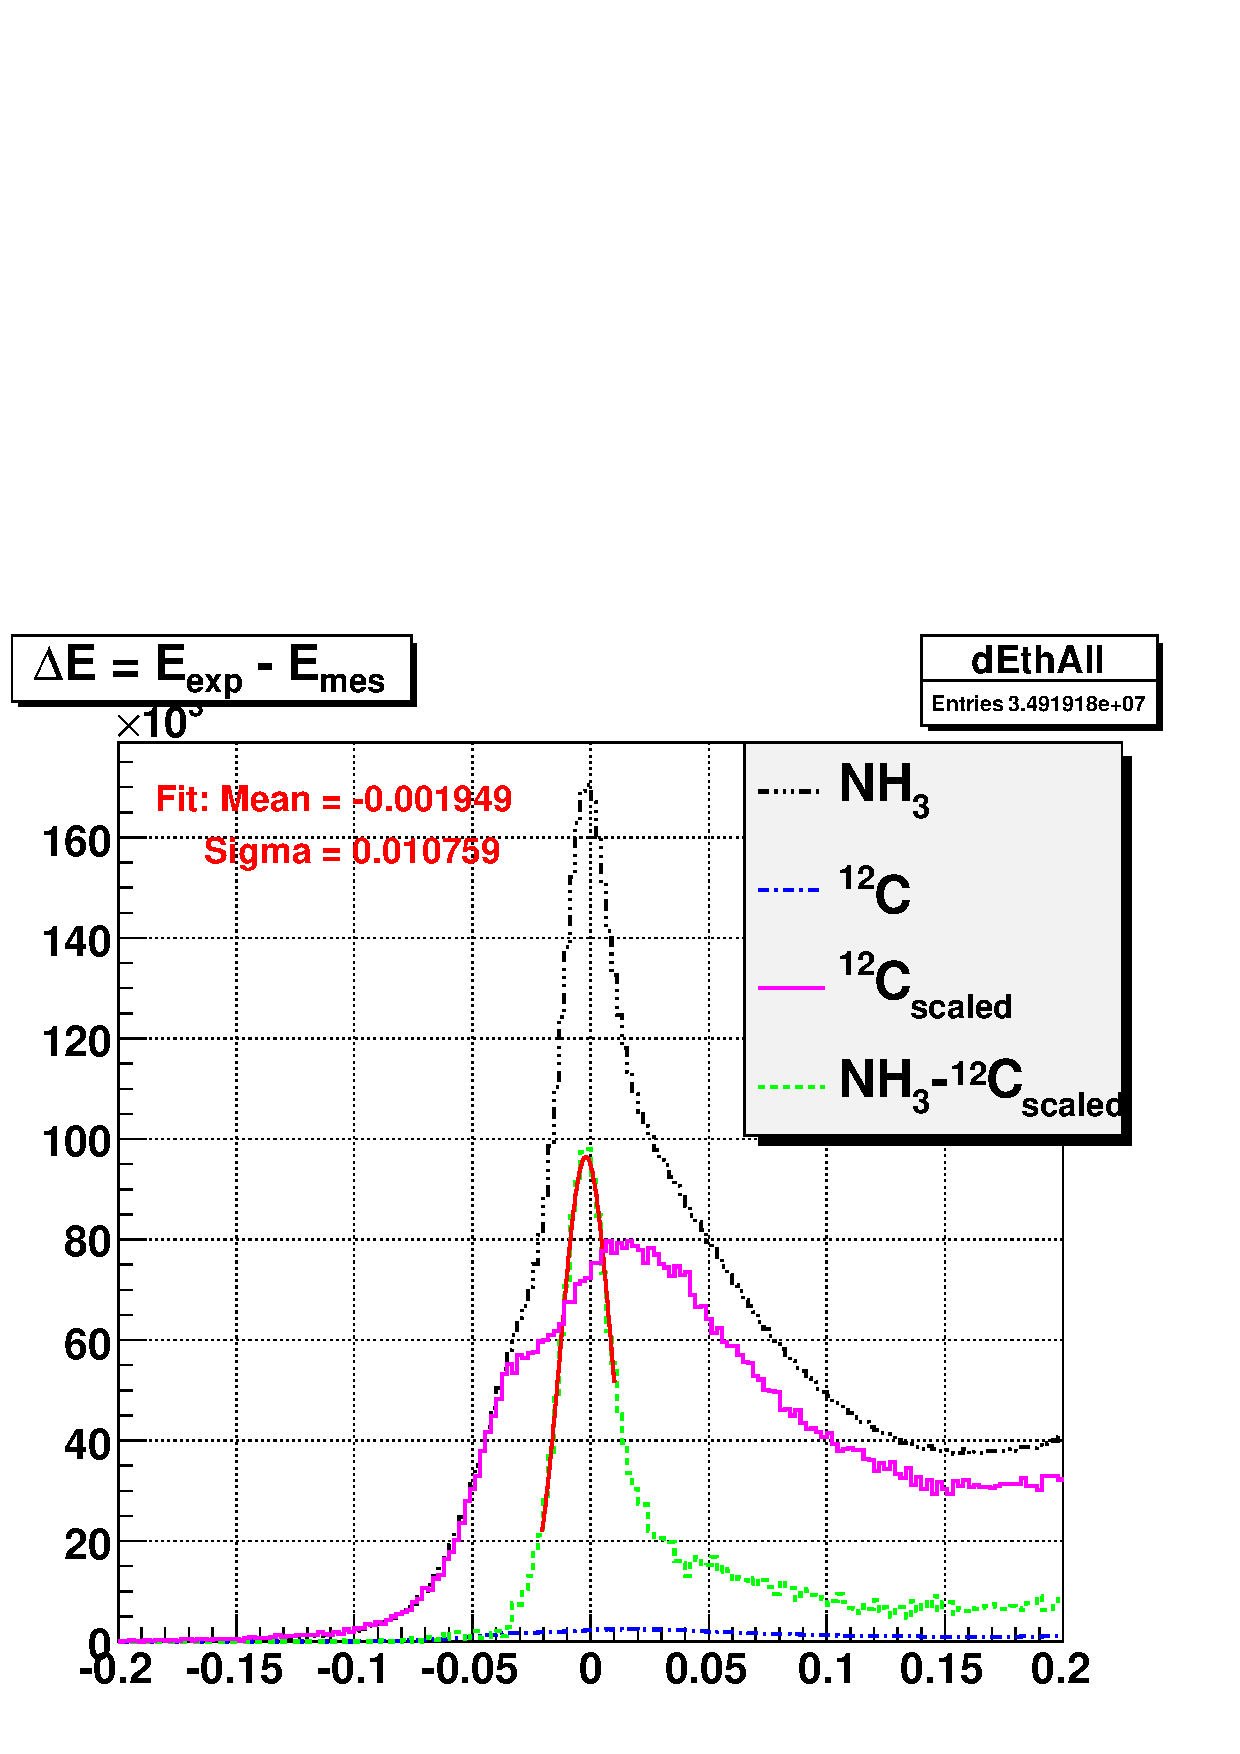
\includegraphics[width=0.8\textwidth]{figuresEG4/FigKineCor/dE_elastProdEb3.png} 
%\centerline{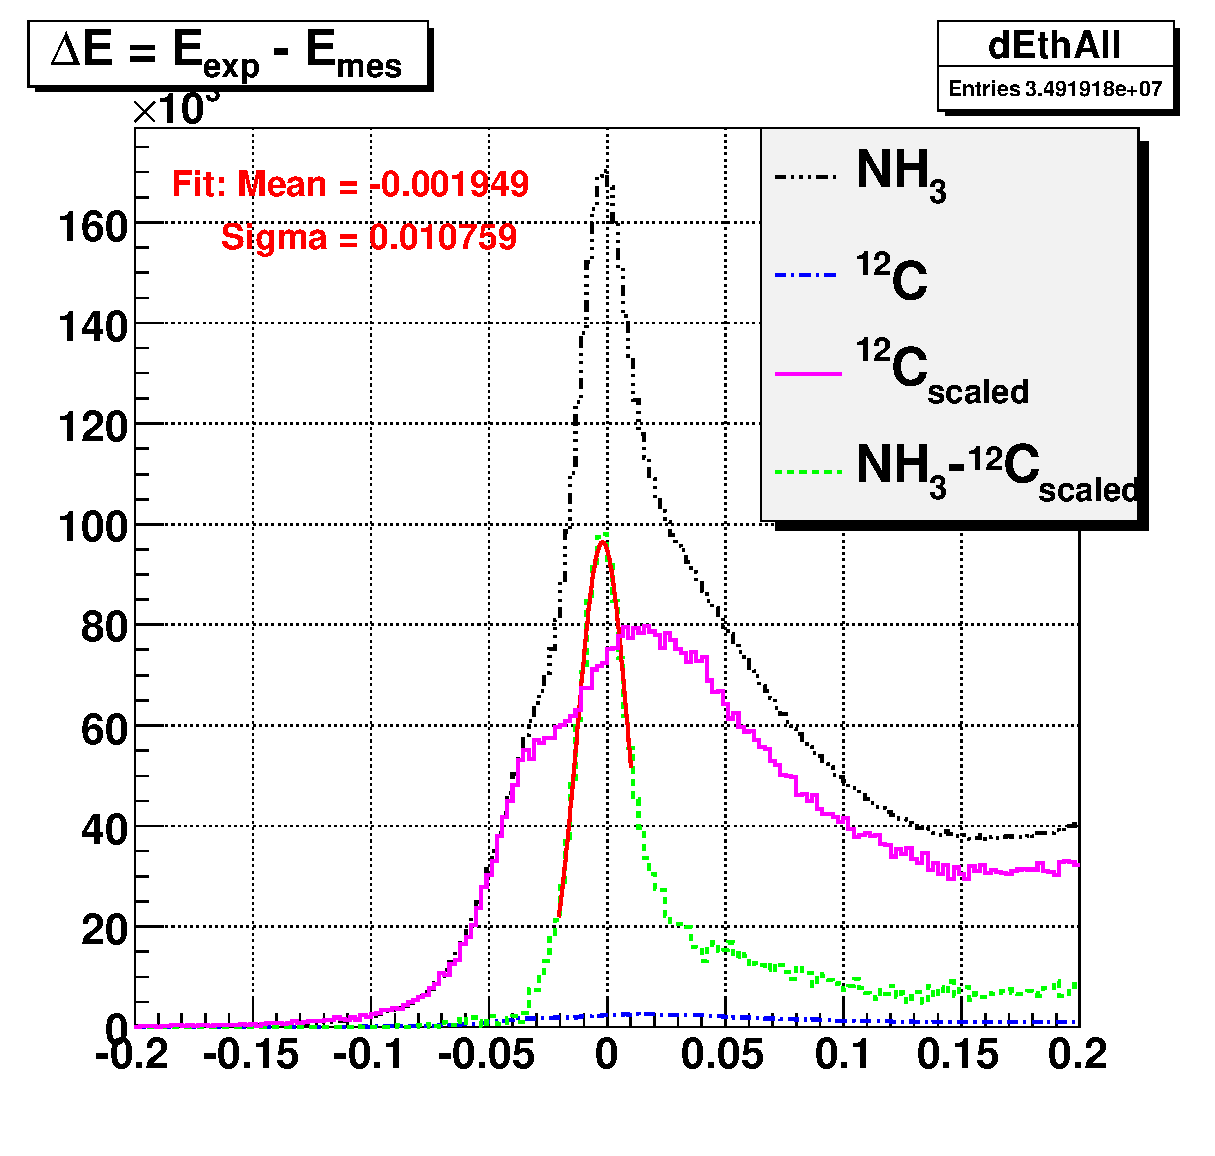
\epsfig{height=10cm,width=15cm,file=chap4simul/DcSmear/dE_elastProdEb3.eps}}
 % \caption[Background subtraction to get elastic peak]{Histograms illustrating the extraction of elastic peak for 2.3 GeV by using 
%carbon-12 data for background removal from the total-cross section (all good electrons with $\theta>7$ used).}
  \caption[Background removal from $\Delta E$]{Plots showing background removal from the $\Delta E$ counts from NH$_3$ 
(shown by ``NH$_3$'' line) data (by subtracting cross-normalized counts from $^{12}$C data (shown by ``$^{12}$C$_{scaled}$'' 
line)) to separate the elastic peak (shown by ``NH$_3$ - $^{12}$C$_{scaled}$'' line) in one of the kinematic bins, thereby 
getting the momentum offset for that bin. The $^{12}$C data is used to account for the nuclear elastic background from $^{15}$N
nucleii in the ammonia target. It would have been best to have data from $^{15}$N target itself but due to technical difficulties
that was not possible and, therefore, $^{12}$C target was chosen as the closest possible approximation of $^{15}$N target.}
  %Some comments on 12C use for 15N background, read page 195 (pdf 210), section IV.11.2 from Nevzat's thesis (my dropbox)
%^{235}_{92}U an example of how an Uranium isotope symbol in Chemistry written with the Latex %kp: April 04, 2010
\label{sec6dEall}
\end{figure}


\begin{figure}[H]%[ht] 
\centering
  \leavevmode \includegraphics[width=0.8\textwidth]{figuresEG4/FigKineCor/elasticPeaksFromNH3wdWoCorEi0mN15gausCropped.png} 
  \caption[Nuclear elastic peak from $^{15}$N target]{Nuclear elastic peaks fron $^{15}$N target and the Gaussian fits in two
of many kinematic bins as seen in $\Delta E = E'_{elastic} - p$ distributions from NH$_3$ data before the momentum corrections.
In this case $E'_{elastic}$ is evaluated using known mass of $^{15}$N in Eq. \ref{eqElasticEprime}.
In the second plot, the proton elastic peak is also visible. Ideally, after all the corrections, the nuclear elastic peak is 
expected to be centered at zero. But, as is obvious from these figures, these peaks show offsets. These offsets (given
by the mean values of the Gaussian fits) are collected from those bins in which the nuclear elastic peaks are very well
separated (particularly the first few angular bins) and used in the $\chi^2$-minimization along with all the offsets of
elastic peaks (see Fig. \ref{sec6dEall})}
\label{sec6dEnucElastEbi0}
\end{figure}



\begin{comment}
\begin{figure}[htpb] %ht, htpb (p - float, b = bottom, h=? t = top)
%\centerline{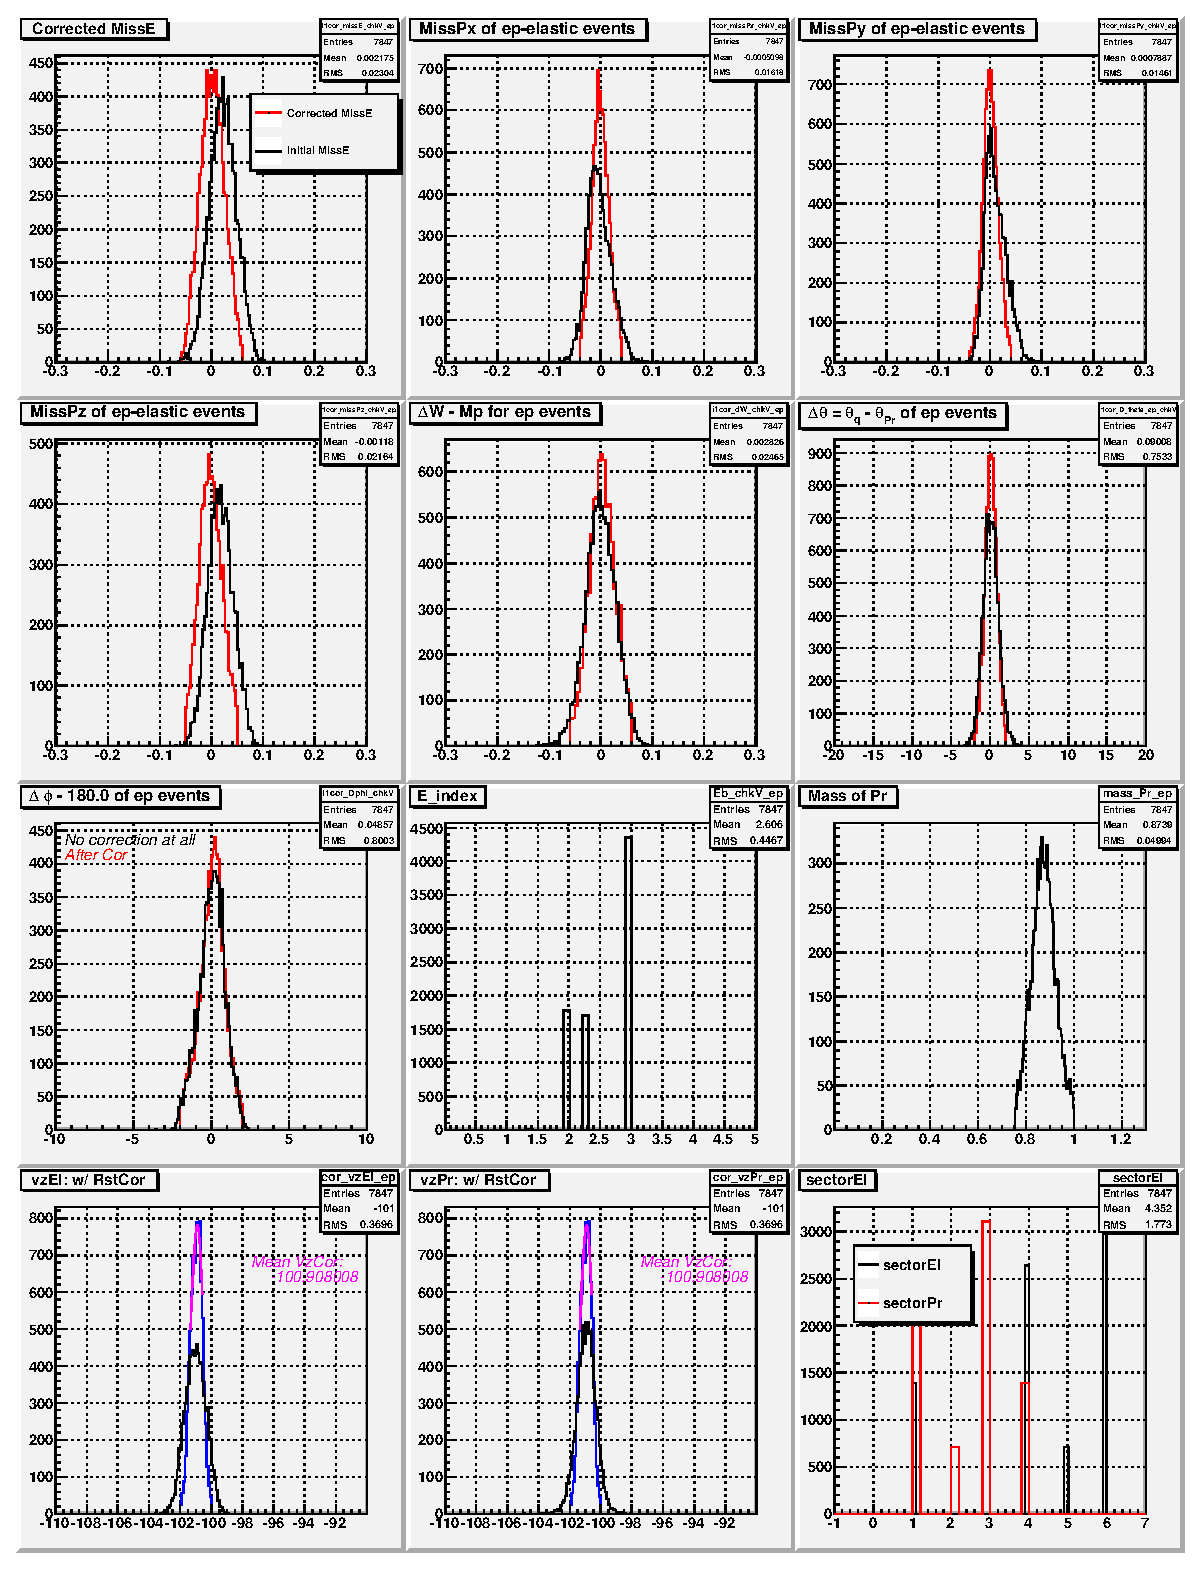
\epsfig{height=20cm,width=15cm,file=chap7KineCor/figures/ep_evntsChkMcor.eps}}
\centering
% \leavevmode 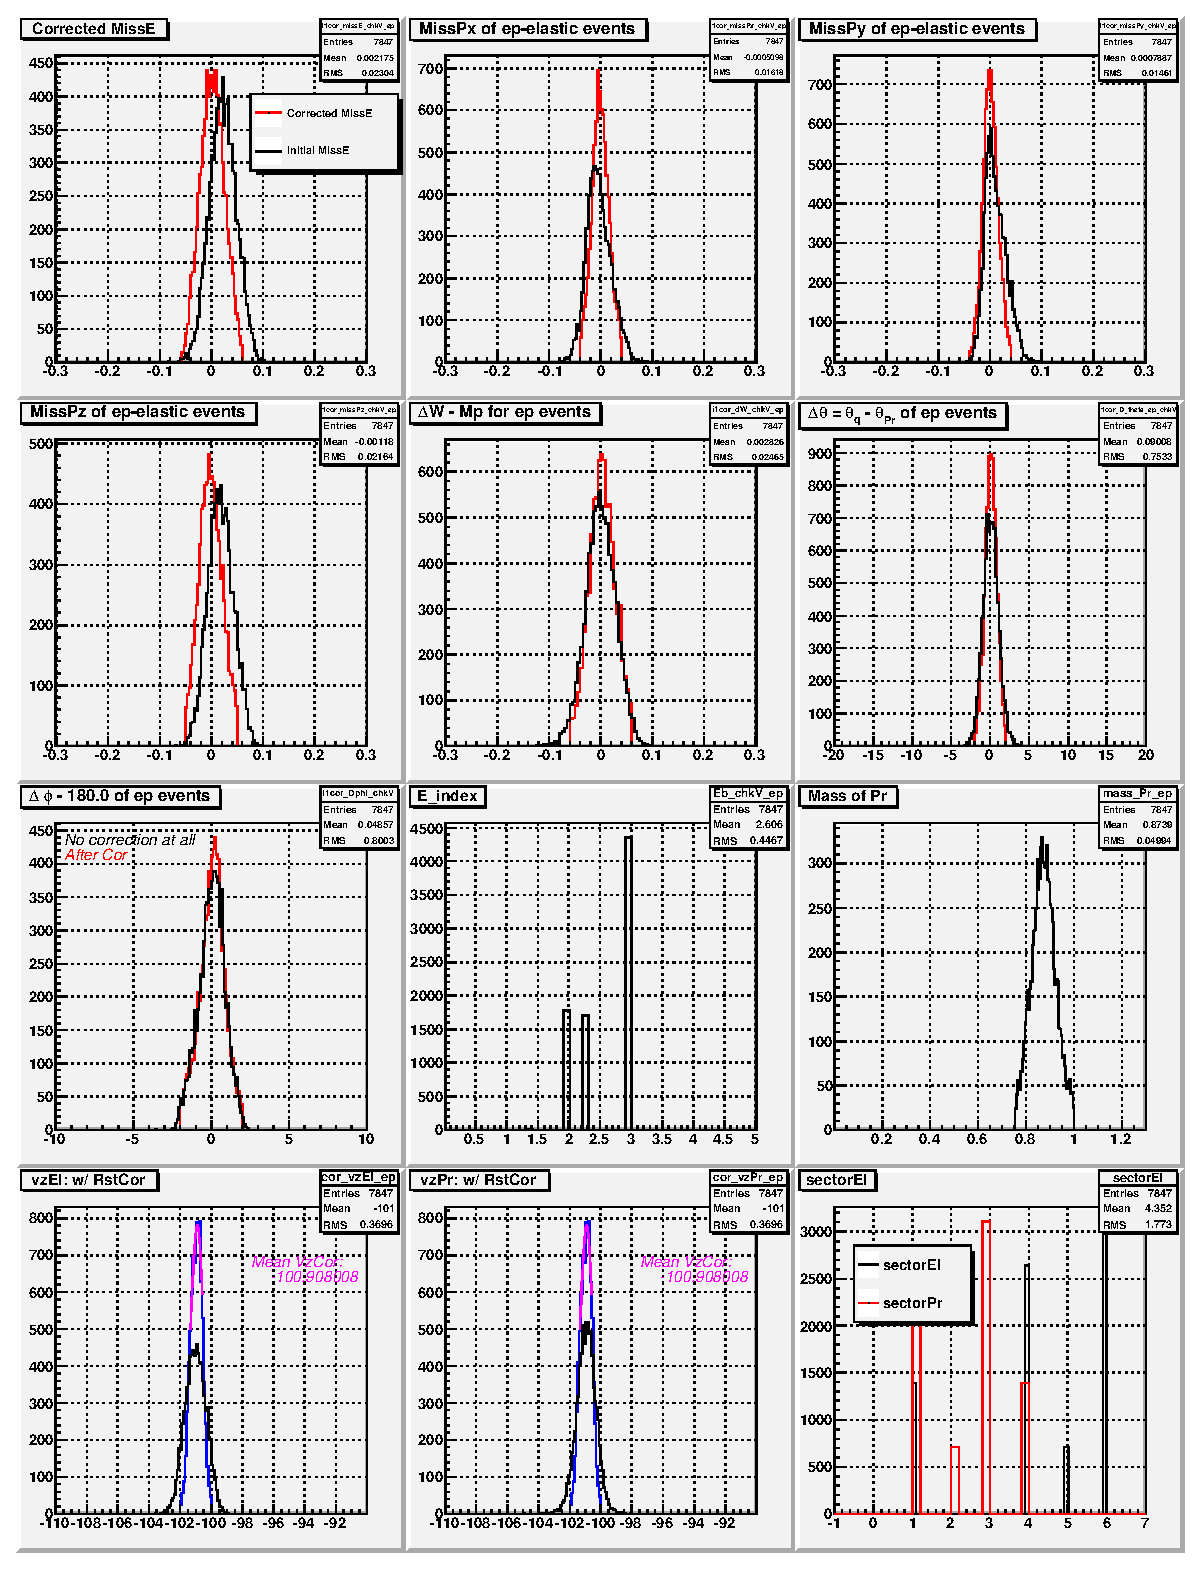
\includegraphics[width=0.85\textwidth]{chap7KineCor/figures/ep_evntsChkMcor.eps} %Used till 11/30/13
%\caption[Effects of corrections ep-elastic events]{Effects of kinematic corrections on ep-elastic events. The first 6 panels 
%show distributions (before ({\bf black}) and after (\textcolor{red}{{\bf red}}) the corrections) of the missing energy, missing 
%(X,Y,Z) components of momenta, $\Delta W = W - M_p$, and $\Delta \theta = \theta_q - \theta_p$, where $\theta_q$ and $\theta_p$ 
%are the expected and measured angles of the recoil proton (or the exchanged virtual photon). The 7th plot is for $\Delta \phi - 180.0$, 
%where $\Delta \phi = \phi_e - \phi_p$. The 10th and 11th plots show the Z-vertex distributions of electrons and protons before 
%({\bf black}) and after (\textcolor{blue}{{\bf blue}}) the corrections.} %Used till 11/30/13
 %\leavevmode 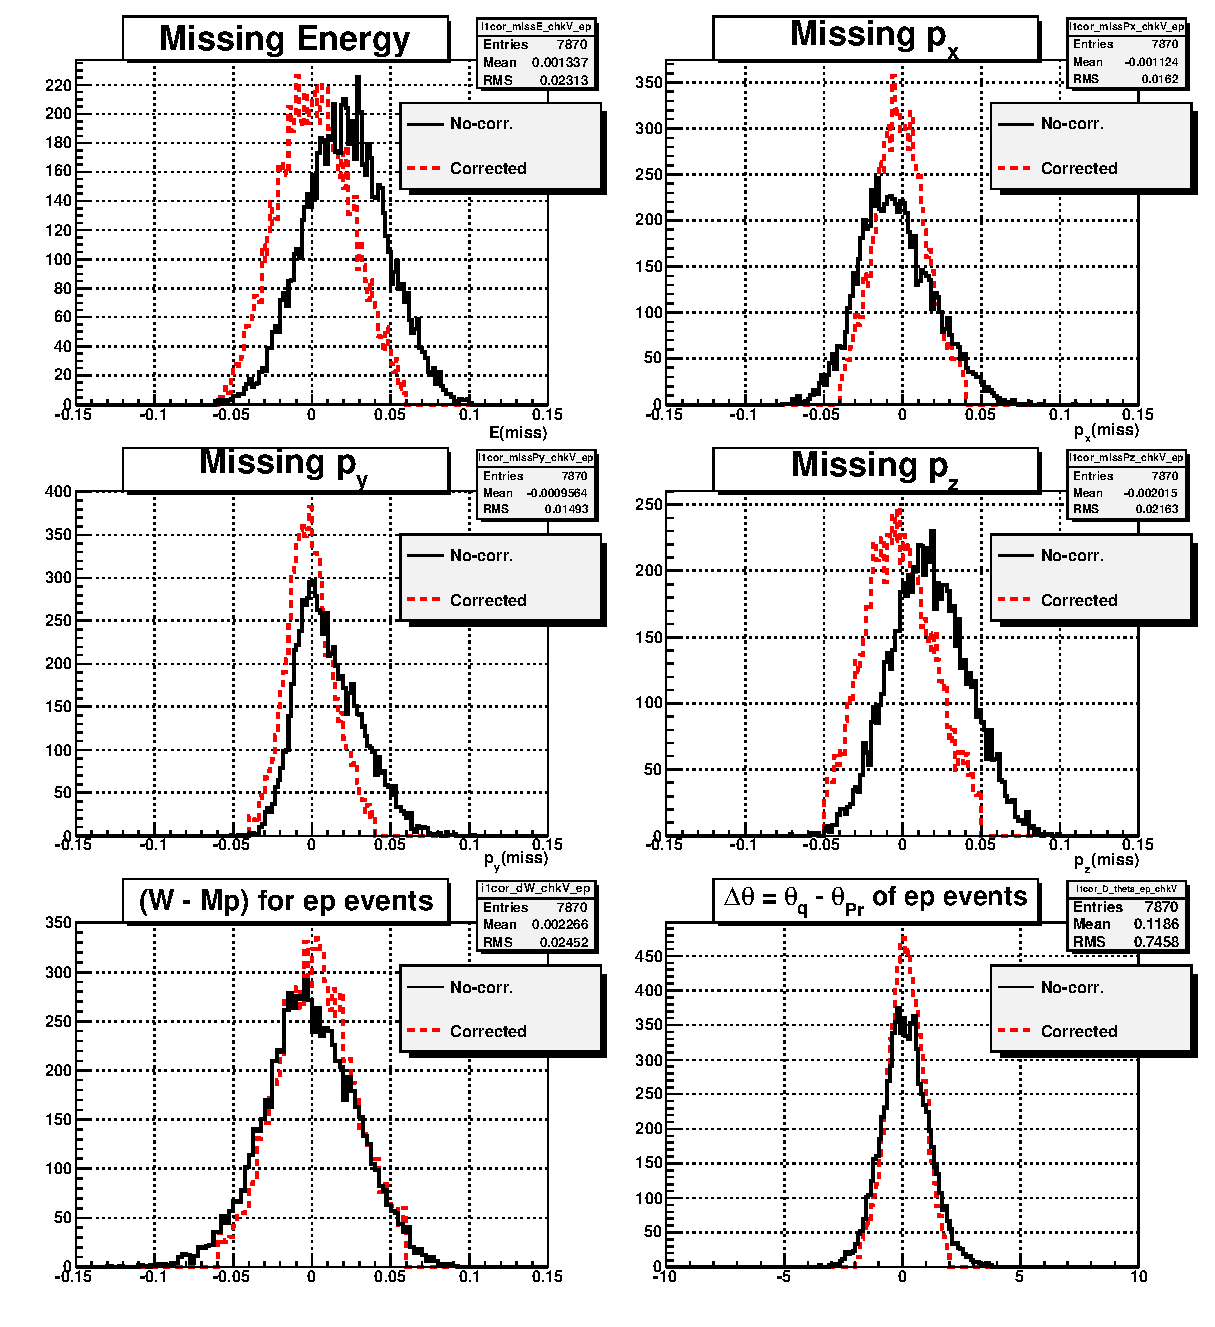
\includegraphics[width=1.0\textwidth]{chap7KineCor/figures/ep_evntsChkMcor2.eps} 
 \leavevmode 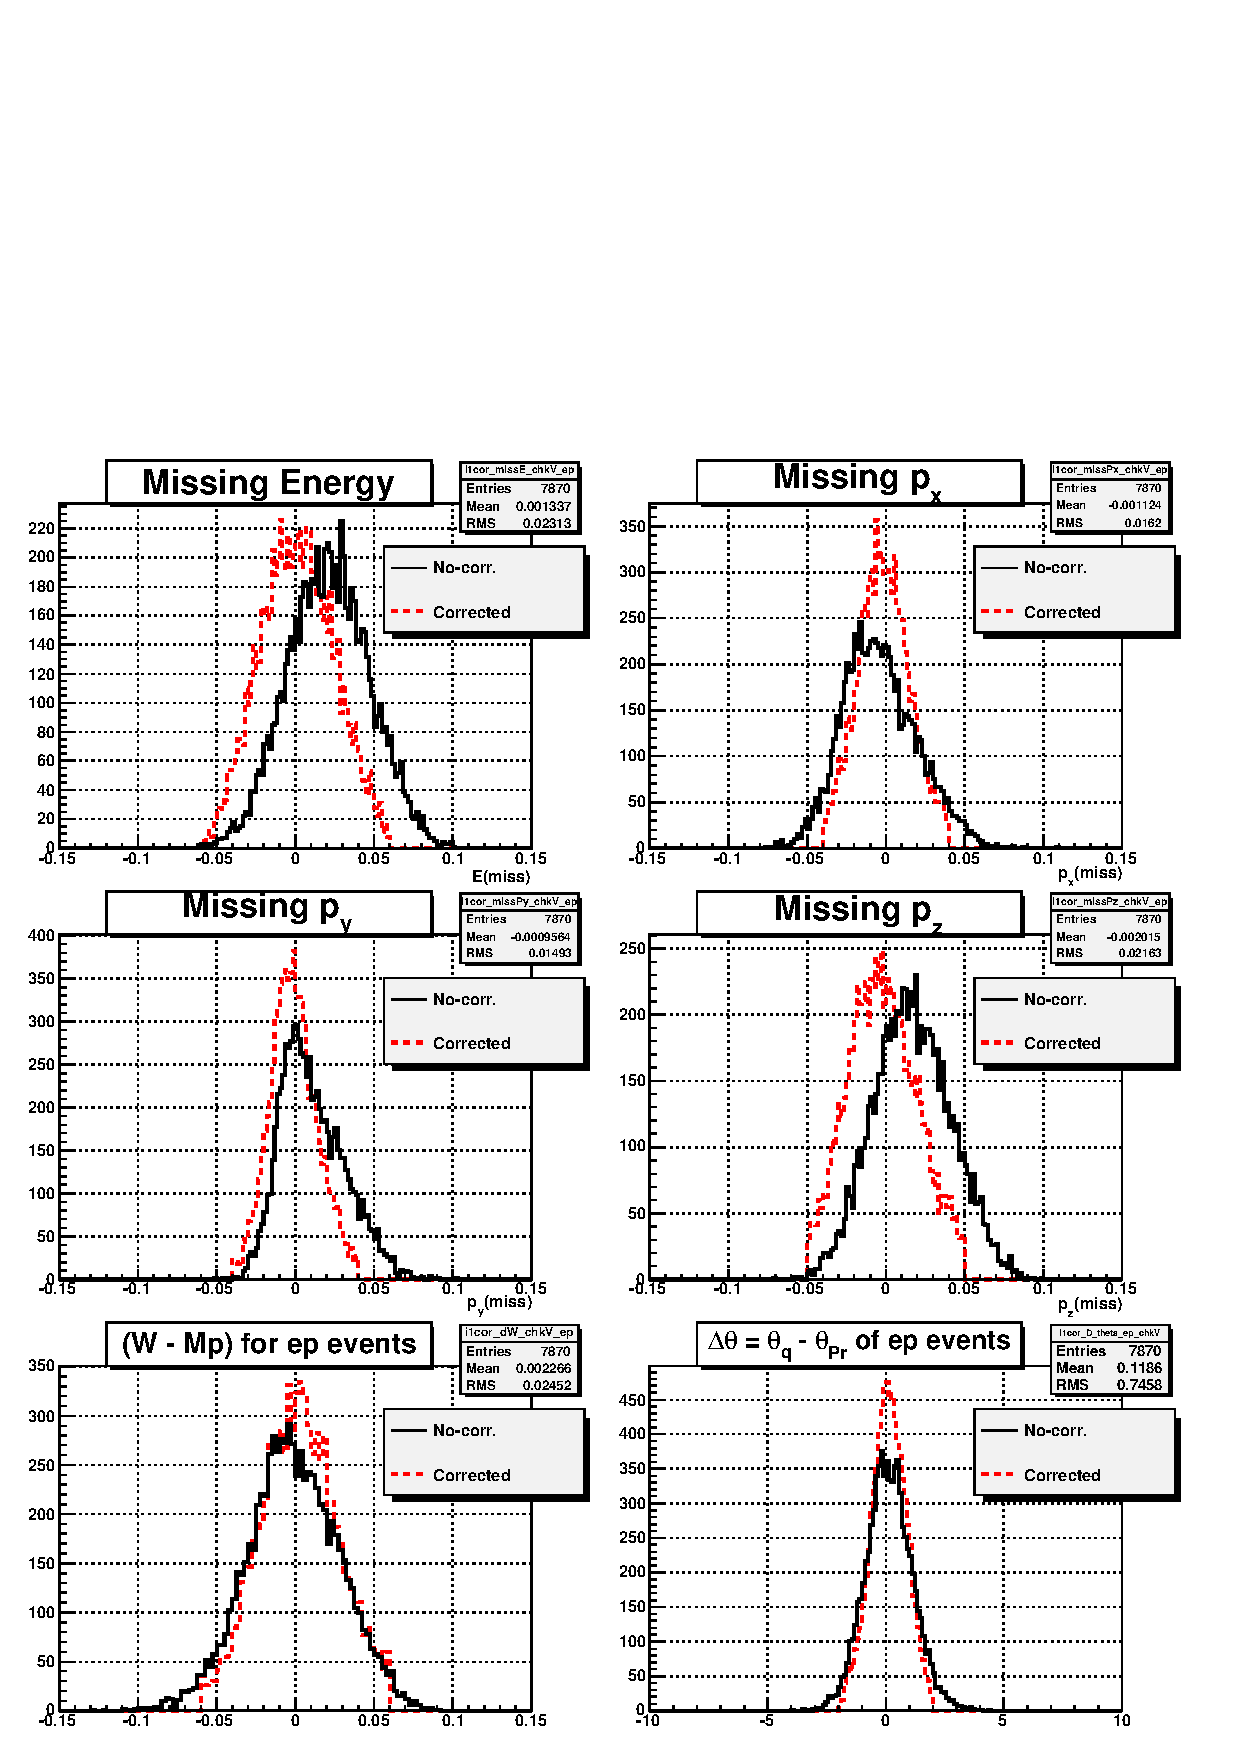
\includegraphics[width=1.0\textwidth]{figuresEG4/FigKineCor/ep_evntsChkMcor2.png} 
\caption[Effects of corrections on ep-elastic events]{Effects of kinematic corrections on ep-elastic events. In the 6 panels the 
distributions of missing energy, missing momentum components ($p_x$, $p_y$, and $p_z$), the difference $\Delta W = W-M_p$ and 
$\Delta \theta = \theta_q - \theta_{p}$ of ep-elastic events respectively. The distributions before the corrections are shown 
by {\bf black continuous} lines and the ones after the corrections are shown by the \textcolor{red}{{\bf red dotted}} lines. 
Here, $M_p$ is the proton mass in GeV. Likewise, $\theta_q$ and $\theta_p$ are the expected and measured angles of the recoil 
proton (or the exchanged virtual photon) respectively. }
\label{fig:epElastic}
\end{figure}
\end{comment}




%\subsection{Correction for the Outgoing Energy Loss due to Ionization}
\subsection{Outgoing Ionization Loss Correction}
\label{secElossCor}
 
%    \sqrt[root]{arg} The \sqrt command produces the square root of its argument. The optional argument, root, determines what root 
%    to produce, i.e., the cube root of x+y  would be typed as  $\sqrt[3]{x+y}$
In addition to the corrections described above, the energy (E) of each of the particles is corrected for the outgoing ionization loss by adding an estimation of ionization loss as follows: $E_{cor} = E + \Delta E $ with $\Delta E = \frac{dE}{dX}\tau$ % $\Delta E = (\frac{\Delta E/\Delta X}{1000.0})gm$,
where the factor $\tau$ is the total effective mass thickness traversed by the particle and
\begin{subequations}
\begin{eqnarray}
\label{eqElossEl}
%\Delta E/ \Delta X = 2.8 ~MeV \quad \rm{for ~electrons}
dE/dX \approx 2.8 ~\rm{MeV/(g ~cm}^{-2}\rm{)} \quad \rm{for ~electrons}
\end{eqnarray}
and, for hadrons \cite{leo1994techniques}
\begin{eqnarray}
\label{eqElossHad}
%%%if( mass < 0.01) DEDX = 2.8;    else DEDX = 0.307 * ( 0.5 / Beta2 ) * ( log( 2. * 511000.0 * Beta2 * ( Gamma2 / 90. ) ) - Beta2 );
%%%\Delta E/ \Delta X = 0.307 (\frac{ 0.5}{ \beta^2}) \left( log\bigg( 2.0( 511000.0 \beta^2) (\frac{ \gamma^2}{ 90.0} ) \bigg) - \beta^2 \right);
%%%\Delta E/ \Delta X = 0.307 (\frac{ 0.5}{ \beta^2}) \left( ln\bigg( 2.0( 511000.0 \beta^2) (\frac{ \gamma^2}{ 90.0} ) \bigg) - \beta^2 \right) ~MeV ~\rm{for ~hadrons} 
%\Delta E/ \Delta X = 0.307 \times \frac{ 0.5}{ \beta^2} \left( ln\bigg( 2.0 \times 511.0 \frac{\beta^2 \gamma^2}{ 0.090} \bigg) - \beta^2 \right) ~MeV 
dE/dX \approx 0.307 \times \frac{ 0.5}{ \beta^2} \left( ln\bigg( 2.0 \times 511.0 \frac{\beta^2 \gamma^2}{ 0.090} \bigg) - \beta^2 \right) \rm{~MeV} 
\end{eqnarray}
\end{subequations}
which is an approximation of the Bethe-Block formula \cite{leo1994techniques}: % (Eq.(\ref{eqBetheBlock})).

\begin{eqnarray}
\label{eqBetheBlock}
-\frac{1}{\rho} \frac{dE}{dx} = 4\pi N_a r_e^2 m_e c^2 \frac{Z}{A} \frac{1}{\beta^2} \left( ln\bigg( \frac{2m_ec^2\gamma^2\beta^2}{I} \bigg) - \beta^2 \right) 
\end{eqnarray}
%And, the factor '$\tau$' is the total effective mass thickness traversed by the particle. 
%This quantity is calculated as follows:
The total effective mass thickness $\tau$ (in cm) is calculated as follows: %xz
\begin{itemize}
\item $\tau = \tau_{\parallel}/cos\theta$ \quad if $\theta <= \pi/4$
\item $\tau = \tau_{\parallel}/cos(\pi/4)$ \quad if $\theta > \pi/4$    %SEK comment:  I don't understand. leave out! Why not \tau = r/sin \theta    (anyway \theta > \pi/4 is never true!
\end{itemize}
where $\tau_{\parallel}$ is calculated as:
\begin{itemize}
\item $\tau_{\parallel} = \Delta z \times 0.6 + 0.4$ \quad if $\Delta z > 0.0 $ and $\Delta z < 1.0 $
\item $\tau_{\parallel} = 0.6 + 0.4$ \quad if $\Delta z \geq  1.0$
\item $\tau_{\parallel} = 0.4$ \quad if $\Delta z \leq  0.0$
%\item $\tau_{\parallel} = 0.75$ \quad if otherwise
\end{itemize}
with $\Delta z = z_{target\_center} - z_{ave} + L_{target}/2 = (-101.0$ cm $ - z_{ave} + 0.5)$ cm being the physical distance (along the target length) traveled by the particle through the polarized target material (e.g. the EG4 ND$_3$ target has length 1.0 cm and is positioned at z = -101.0 cm). The factor 0.6 is the effective mass thickness of ND$_3$ (density of ND$_3$ ($\sim 1 ~g/cm^3$) %(e.g. one of the EG4 NH$_3$ (ND$_3$ too) target has length 1.0 cm and is positioned at z = -101.0 cm). The factor 0.6 is the effective mass thickness of NH$_3$ (density of NH$_3$ ($\sim 1 ~g/cm^3$) 
multiplied by the packing fraction which is roughly 0.6  \cite{rferschAnaNote},%{rfersch_th},
whereas 0.4 is the sum of the mass thicknesses of He ($\sim 0.3$) and that of window foils ($\sim 0.1$) \cite{nGuler_th}. %In fact these numbers were for NH3 targets and were decided when our own values for PFs were not available which are now at about 0.7 (I believe, this won't make things much different, may be systematic study has to be done. 12/5/13)


% double zcenter    = -101.0; //-55.1;//#ignore
%  double \Delta z = zcenter - zave + 0.5;//#ignore
%  //kp:  \Delta z is the fraction of the distance the particle travelled i.e. \Delta z = (zave - zcenter + 0.5)/Lt  (Lt = target length = 1.0 for EG1B)
%  //     (denoted by delta_z in Nevzat's thesis), also in thesis, the order of zave -zcenter is wrong.
%  double E = sqrt(p*p + mass*mass);
%  double fbeta = p/E;  double Beta2 = fbeta * fbeta; double Gamma2 = 1.0 / ( 1.0 - Beta2 );  
    
%    if( ( \Delta z <= 1.0 ) && ( \Delta z >= 0.0 ) )  \tau = \Delta z * 0.6 + 0.4;
%    //kp: I think \tau is total effective mass thickness traversed by the particle
%    //    The factor 0.6 is effective mass thickness of NH$_3$ (density of NH$_3$ (about 1 g/cm^3) multiplied by the packing fraction which is 
%    //    roughly 0.6; See R. Fersch's thesis at page 215) and 0.4 is the sum of 0.3 and 0.1 where
%    //    0.4 is for mass thickness of He and 0.1 for that of window foils (see Nevzat's thesis, page 158)

%    else if( \Delta z >= 1.0 )  \tau = 0.6 + 0.4;
%    else if( \Delta z <= 0.0 )  \tau = 0.4;
%    else  \tau = 0.75;
%   //Ignore all above lines with '#ignore' and use '\tau = 0.75' for all cases for a reasonable approximation (Dr. Kuhn)
    
%    if( theta * rad2deg <= 45. ) \tau = \tau / cos( theta );
%    else  \tau = \tau / cos( 45. * deg2rad );

Using the ionization loss corrected energy and the rest mass of the particle, momentum is recalculated as $p_{cor} = \sqrt{E^2_{cor}-m^2}$ 
(where $m$ is the mass of the particle). Finally, this new p is used along with the previously corrected angles to evaluate the three 
cartesian components $p_x$, $p_y$ and $p_z$ of the momentum as follows:

\begin{equation}
\begin{aligned}
  p_x   = & p \sin\theta \cos\phi \\
  p_y   = & p \sin\theta \sin\phi \\
  p_z   = & p \cos\theta 
\end{aligned}
\end{equation}




\begin{figure}[htpb] %ht, htpb (p - float, b = bottom, h=? t = top)
%\centerline{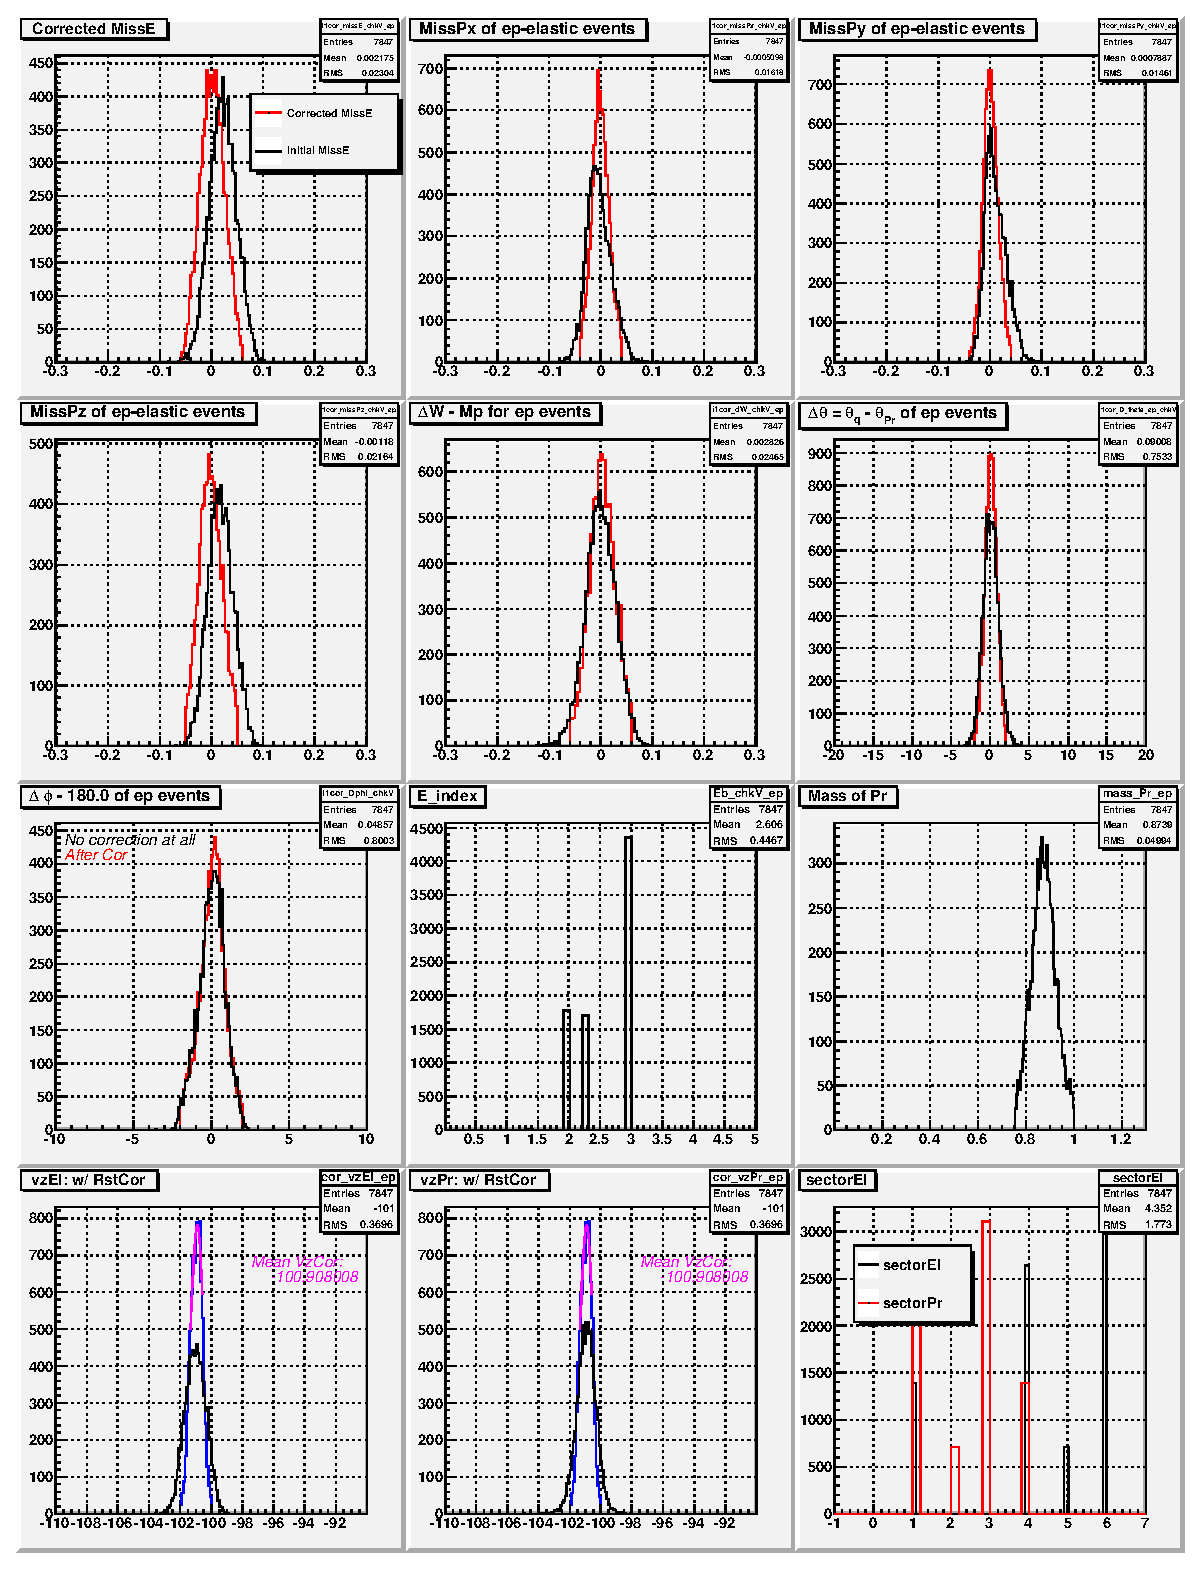
\epsfig{height=20cm,width=15cm,file=chap7KineCor/figures/ep_evntsChkMcor.eps}}
\centering
 \leavevmode \includegraphics[width=1.0\textwidth]{TexmakerMyFinTh/chap7KineCor/figures/momCorTestInclEi4Pass2Pars11N15_18pTC.png} 
\caption[Effects of corrections on inclusive events from 3 GeV NH$_3$ data]{Effects of kinematic corrections on inclusive events 
from 3 GeV NH$_3$ data. Here, distributions of $\Delta E$ and $W$ are shown in two different ranges. The upper ones shown the full 
range distributions, where as the lower two show the distributions near the quasi-elastic peak. The distributions before the 
corrections are shown by {\bf black continuous} lines and the ones after the corrections are shown by the \textcolor{red}{{\bf red}} 
lines. Here, $E_{elast}$ is the calculated or expected energy of the scattered electron assumming it was scattered off
elastically, whereas, p[0] is the momentum as measured by CLAS. From these plots it is evident that the momentum correction works
as expected because the peak of $\Delta E$ is narrower and better centered at zero after the correction.}
\label{fig:epElastic}
\end{figure}



